%%%%%%%%%%%%%%%%%% PREAMBULE %%%%%%%%%%%%%%%%%%

\documentclass[11pt,a4paper]{article}

\usepackage{amsfonts,amsmath,amssymb,amsthm}
\usepackage[utf8]{inputenc}
\usepackage[T1]{fontenc}
\usepackage[french]{babel}
\usepackage{fancybox}
\usepackage{graphicx}
%\usepackage{tikz}

%----- Ensembles : entiers, reels, complexes -----
\newcommand{\Nn}{\mathbb{N}} \newcommand{\N}{\mathbb{N}}
\newcommand{\Zz}{\mathbb{Z}} \newcommand{\Z}{\mathbb{Z}}
\newcommand{\Qq}{\mathbb{Q}} \newcommand{\Q}{\mathbb{Q}}
\newcommand{\Rr}{\mathbb{R}} \newcommand{\R}{\mathbb{R}}
\newcommand{\Cc}{\mathbb{C}} \newcommand{\C}{\mathbb{C}}
\newcommand{\Kk}{\mathbb{K}} \newcommand{\K}{\mathbb{K}}

%----- Modifications de symboles -----
\renewcommand{\epsilon}{\varepsilon}
\renewcommand{\Re}{\mathop{\mathrm{Re}}\nolimits}
\renewcommand{\Im}{\mathop{\mathrm{Im}}\nolimits}
\newcommand{\llbracket}{\left[\kern-0.15em\left[}
\newcommand{\rrbracket}{\right]\kern-0.15em\right]}
\renewcommand{\ge}{\geqslant} \renewcommand{\geq}{\geqslant}
\renewcommand{\le}{\leqslant} \renewcommand{\leq}{\leqslant}

%----- Fonctions usuelles -----
\newcommand{\ch}{\mathop{\mathrm{ch}}\nolimits}
\newcommand{\sh}{\mathop{\mathrm{sh}}\nolimits}
\renewcommand{\tanh}{\mathop{\mathrm{th}}\nolimits}
\newcommand{\cotan}{\mathop{\mathrm{cotan}}\nolimits}
\newcommand{\Arcsin}{\mathop{\mathrm{arcsin}}\nolimits}
\newcommand{\Arccos}{\mathop{\mathrm{arccos}}\nolimits}
\newcommand{\Arctan}{\mathop{\mathrm{arctan}}\nolimits}
\newcommand{\Argsh}{\mathop{\mathrm{argsh}}\nolimits}
\newcommand{\Argch}{\mathop{\mathrm{argch}}\nolimits}
\newcommand{\Argth}{\mathop{\mathrm{argth}}\nolimits}
\newcommand{\pgcd}{\mathop{\mathrm{pgcd}}\nolimits} 

%----- Structure des exercices ------
%\theoremstyle{definition}

\newtheoremstyle{exostyle}
{15pt}
{15pt}
{\normalfont}
{0pt}
{\bfseries}
{}
{\newline}
{\thmname{#1}~\thmnumber{#2} -- \thmnote{#3}}
\theoremstyle{exostyle} 

\newtheorem{exo}{Exercice}
\newtheorem{ind}{Indications}
\newtheorem{cor}{Correction}

\newcommand{\exercice}[1]{} \newcommand{\finexercice}{}
%\newcommand{\exercice}[1]{{\tiny\texttt{#1}}\vspace{-2ex}} % pour afficher le numero absolu, l'auteur...
\newcommand{\enonce}{\begin{exo}} \newcommand{\finenonce}{\end{exo}}
\newcommand{\indication}{\begin{ind}} \newcommand{\finindication}{\end{ind}}
\newcommand{\correction}{\begin{cor}} \newcommand{\fincorrection}{\end{cor}}

\newcommand{\noindication}{\stepcounter{ind}}
\newcommand{\nocorrection}{\stepcounter{cor}}

\newcommand{\fiche}[1]{} \newcommand{\finfiche}{}
\newcommand{\titre}[1]{\centerline{\large \bf #1}}
\newcommand{\addcommand}[1]{}
\newcommand{\video}[1]{}

%----- Presentation ------
\setlength{\parindent}{0cm}

\newcommand{\ExoSept}{\textbf{\textsf{Exo7}}}
\newcommand{\LogoExoSept}{\setlength{\unitlength}{0.6em}
	\begin{picture}(0,0)  \thicklines     \put(0,4){\line(0,1){3}}   \put(0,7){\line(1,0){3}}
		\put(3,7){\line(0,-1){7}}  \put(0,4){\line(1,0){7}}   \put(3,0){\line(1,0){4}}
		\put(7,0){\line(0,1){4}}   \put(3,7){\line(4,-3){4}}  \put(7,4){\line(3,4){3}}  
		\put(10,8){\line(-4,3){4}} \put(3,7){\line(3,4){3}}   \put(4.6,6.8){\mbox{\ExoSept}}
\end{picture}}

%----- Commandes supplementaires ------

\usepackage[a4paper, margin = 2cm]{geometry}
\usepackage[charter]{mathdesign}
%\usepackage{import}

\usepackage{tikz}
\usetikzlibrary{calc,shadows,arrows,shapes,patterns,matrix}
\usetikzlibrary{decorations.pathmorphing}
\usetikzlibrary{fadings}
\usetikzlibrary{external}
\usetikzlibrary{positioning}
\usetikzlibrary{arrows}
\usetikzlibrary{backgrounds}
\usepackage{tikz,tikz-3dplot}

\newcommand{\sauteligne}{\leavevmode\vspace{-\baselineskip}}

\begin{document}

	
	
%%%%%%%%%%%%%%%%%% ENTETE %%%%%%%%%%%%%%%%%%



%\kern-2em
\textsc{Feuille d'exercices 1}\hfill\textsc{Fonctions de plusieurs variables}

\vspace*{0.5ex}
\hrule\vspace*{1.5ex} 
\hfil{\textbf{\Large \textsc{Fonctions de plusieurs variables}}}
\vspace*{1ex} \hrule 
\vspace*{5ex} 



%-------------------------------------------
\section{Graphe \& co}

\exercice{}
\enonce[Une fonction de deux variables]
Soit $f$ la fonction définie par :
$$f(x,y) = x^4 -4x^2y + 6y^2$$
\begin{enumerate}
	\item Calculer $f(1,-2)$.
	\item Calculer $f(x,x)$.
	\item Calculer $f\left(\frac1y,\frac{y}{x^2}\right)$.
	\item Exprimer $f(tx,t^2y)$ en fonction de $t$ et $f(x,y)$.
	\item Montrer que $f(x,y) \ge 0$ en exprimant $f(x,y)$ comme somme de deux carrés.
	\item Résoudre $f(x,y)=0$.
\end{enumerate}
\finenonce

\indication
Pour la positivité de $f$ : $x^4 -4x^2y + 6y^2 = (x^2-2y)^2 + 2y^2$.
\finindication

\correction
\begin{enumerate}
	\item $f(1,-2) = 33$.
	\item $f(x,x) = x^4 - 4x^3 + 6x^2$.
	\item $f\left(\frac1y,\frac{y}{x^2}\right) = \frac{1}{y^4} - \frac{4}{x^2y} + \frac{6y^2}{x^4}$.
	\item $f(tx,t^2y) = t^4 f(x,y)$.
	\item On reconnaît dans $x^4 -4x^2y$ le début du carré développé $(x^2-2y)^2$.
	Ainsi $f(x,y) = x^4 -4x^2y + 6y^2 = (x^2-2y)^2 + 2y^2$.
	Cela prouve $f(x,y) \ge 0$ quels que soient $x,y \in \Rr$ car la somme de deux carrés est toujours positive.
	\item Pour que cette somme de carrés soit égale à \(0\), chaque terme doit être nul.
	Donc d'une part \( 2y^2 = 0 \) et donc \( y = 0 \).
	D'autre part \( (x^2 - 2y)^2 = 0 \), mais comme \(y=0\), alors  \( x = 0 \).
	Ainsi, la seule solution de \( f(x,y) = 0 \) est \( (x,y) = (0,0) \).
\end{enumerate}
\fincorrection

\finexercice
	
	
\exercice{}
\enonce[Domaine de définition]
Déterminer, puis représenter, le domaine de définition des fonctions suivantes.
\begin{enumerate}
	\item $f(x,y) = \sqrt{x^2 + y^2 - 4}$
	\item $f(x,y) = \ln(xy+1)$
	\item $f(x,y) = \frac{x^2 - \sin(y)}{x^2+y^2}$
	\item $f(x,y) = \frac{\sqrt{xy}}{x^2+y}$
	\item $f(x,y) = \arcsin(|x| + y)$		
	\item $f(x,y,z) = \frac{1}{3x-2y+z-1}$	
	\item $f(x,y,z) = \sqrt{x} + \sqrt{1-y^2} + \sqrt{z-1}$	
\end{enumerate}
\finenonce

\indication
Il faut connaître l'équation d'un cercle, d'une droite, d'une parabole, d'une hyperbole, d'un plan...

Il peut aussi être plus facile de déterminer et dessiner les points interdits que les points autorisés.
\finindication

\correction
\begin{enumerate}
	\item $f(x,y) = \sqrt{x^2 + y^2 - 4}$.
	
	Il faut $x^2+y^2-4 \ge 0$. On sait que $x^2+y^2-4 = 0$ est l'équation du cercle de centre $(0,0)$ et de rayon $2$. Les points $(x,y)$ qui vérifient  $x^2+y^2-4 \ge 0$ sont ceux à l'extérieur de ce cercle (y compris les points du cercle).
	
	Dans les dessins ci-dessous on représente en vert le domaine de définition et en rouge le complémentaire (là où la fonction n'est pas définie).
	
\begin{center}
	\small
	\begin{minipage}{0.3\textwidth}	
			\begin{tikzpicture}[scale=0.5]
			
			\fill[green!70!black!40] (-4,-4) rectangle (4,4);
			\fill[red!10] (0,0) circle (2);		
			
			\draw[->,>=latex, gray] (-4.2,0)--(4.5,0) node[below,black] {$x$};
			\draw[->,>=latex, gray] (0,-4.2)--(0,4.5) node[right,black] {$y$};
			
			
			\draw[green!70!black,ultra thick] (0,0) circle (2);
			
			\fill (0,0) circle (1pt);
			\node at (45:2)[above right] {$\mathcal{C}$};
			\node at (2,0)[below left] {$2$};		
			\node at (0,0)[below right] {$0$};
			\node at (2.5,-2){$\mathcal{D}_f$};
			
			\node at (0,-5) {$f(x,y) = \sqrt{x^2 + y^2 - 4}$};
		\end{tikzpicture}
	\end{minipage}
	\begin{minipage}{0.3\textwidth}	
			\begin{tikzpicture}[scale=0.5]
			
			\fill[green!70!black!40] (-4,-4) rectangle (4,4);
			%		\fill[red!10] (0,0) circle (2);		
			
			\draw[->,>=latex, gray] (-4.2,0)--(4.5,0) node[below,black] {$x$};
			\draw[->,>=latex, gray] (0,-4.2)--(0,4.5) node[right,black] {$y$};
			
			
			\fill[ultra thick, color=red!10,domain=0.25:4,samples=100,smooth] plot (\x,-1/\x) -- (4,-4) --cycle;		
			\fill[ultra thick, color=red!10,domain=0.25:4,samples=100,smooth] plot (-\x,1/\x) -- (-4,4) --cycle;				
			
			\draw[ultra thick, color=red!70,domain=0.25:4,samples=100,smooth] plot (\x,-1/\x);	
			\draw[ultra thick, color=red!70,domain=0.25:4,samples=100,smooth] plot (-\x,1/\x);	
			\fill[ultra thick, color=red!10,domain=0.25:4,samples=100,smooth] plot (\x,-1/\x) -- (4,-4) --cycle;			
			\fill (0,0) circle (1pt);	
			\node at (0,0)[below right] {$0$};
			\node at (2.5,2){$\mathcal{D}_f$};
			
			\node at (0,-5) {$f(x,y) =  \ln(xy+1)$};
		\end{tikzpicture}
\end{minipage}	
	\begin{minipage}{0.3\textwidth}	
			\begin{tikzpicture}[scale=0.5]
			
			\fill[green!70!black!40] (-4,-4) rectangle (4,4);
			
			
			\draw[->,>=latex, gray] (-4.2,0)--(4.5,0) node[below,black] {$x$};
			\draw[->,>=latex, gray] (0,-4.2)--(0,4.5) node[right,black] {$y$};
			
			
			\fill[red] (0,0) circle (6pt);	
			\node at (0,0)[below right] {$(0,0)$};
			\node at (2.5,2){$\mathcal{D}_f$};
			
			\node at (0,-5) {$f(x,y) =  \frac{x^2 - \sin(y)}{x^2+y^2}$};
		\end{tikzpicture}
\end{minipage}
\end{center}
		
			
	\item $f(x,y) = \ln(xy+1)$.
	
	Il faut $xy+1>0$. On sait que $xy+1=0$ est l'équation d'une hyperbole (comme $xy=-1$, c'est le graphe de la fonction $x \mapsto y = -\frac{1}{x}$). La région $xy+1>0$ est donc délimitée par cette hyperbole ; pour savoir de quel côté elle est située on teste avec des points particuliers. Par exemple $(0,0)$ vérifie bien $xy+1>0$. Donc $\mathcal{D}_f$ correspond à la zone entre les branches de l'hyperbole.
	
	\item $f(x,y) = \frac{x^2 - \sin(y)}{x^2+y^2}$.
	
	La seule condition vient du dénominateur qui ne doit pas s'annuler. Mais $x^2+y^2=0$ si et seulement si $(x,y)=(0,0)$. Le domaine de définition est donc le plan privé de l'origine.
	
	
	\item $f(x,y) = \frac{\sqrt{xy}}{x^2+y}$.
	
	Il faut d'une part $xy\ge0$, c'est-à-dire être dans le quadrant $(x\ge0,y\ge0)$ ou le quadrant $(x\le0,y\le0)$ et d'autre part $x^2+y \neq 0$, c'est-à-dire ne pas être sur la parabole d'équation $y=-x^2$.
\begin{center}
	\small
	\begin{minipage}{0.3\textwidth}	
		\begin{tikzpicture}[scale=0.5]	
	\fill[green!70!black!40] (-4,-4) rectangle (4,4);
	\fill[red!10] (-4,4) rectangle (0,0);
	\fill[red!10] (4,-4) rectangle (0,0);
	
	%		\fill[red!10] (0,0) circle (2);		
	
	\draw[->,>=latex, gray] (-4.2,0)--(4.5,0) node[below,black] {$x$};
	\draw[->,>=latex, gray] (0,-4.2)--(0,4.5) node[right,black] {$y$};	
	
	\draw[ultra thick, color=red!70,domain=-2:2,samples=100,smooth] plot (\x,-\x*\x);	
	
	\fill (0,0) circle (1pt);	
	\node at (0,0)[above right] {$0$};
	\node at (2.5,2){$\mathcal{D}_f$};
	
	\node at (0,-5) {$f(x,y) =  \frac{\sqrt{xy}}{x^2+y}$};
\end{tikzpicture}
\end{minipage}	
\begin{minipage}{0.3\textwidth}	
	\begin{tikzpicture}[scale=1]
		\fill[red!10] (-2,-2) rectangle (2,2);			
		\fill[green!70!black!40] (-2,-2) -- (-2,-1) -- (0,1) -- (2,-1) -- (2,-2) -- (1,-2) -- (0,-1) -- (-1,-2) -- cycle;
		
		%		\fill[red!10] (-4,4) rectangle (0,0);
		%		\fill[red!10] (4,-4) rectangle (0,0);
		
		%		\fill[red!10] (0,0) circle (2);		
		
		\draw[->,>=latex, gray] (-2.2,0)--(2.5,0) node[below,black] {$x$};
		\draw[->,>=latex, gray] (0,-2.2)--(0,2.5) node[right,black] {$y$};
		
		
		
		\draw[color=black!70, dashed] (-1,2) --(2,-1) node[right,scale=0.8]{$x+y=1$};
		\draw[color=green!70!black, ultra thick] (0,1) --(2,-1);
		
		\draw[color=black!70, dashed] (-2,1) --(1,-2) node[below right,scale=0.8]{$x+y=-1$};
		\draw[color=green!70!black, ultra thick] (0,-1) --(1,-2);
		
		\draw[color=black!70, dashed] (1,2) --(-2,-1) node[left,scale=0.8]{$-x+y=1$};
		\draw[color=green!70!black, ultra thick] (0,1) --(-2,-1);
		
		\draw[color=black!70, dashed] (2,1) --(-1,-2) node[below left,scale=0.8]{$-x+y=-1$};
		\draw[color=green!70!black, ultra thick] (0,-1) --(-1,-2);
		
		
		\fill (0,0) circle (2pt);	
		\node at (0,0)[above right] {$0$};
		\fill (1,0) circle (2pt);	
		\node at (1,0)[above right] {$1$};
		\fill (0,1) circle (2pt);	
		\node at (0,1)[above right] {$1$};
		
		\node at (1.5,-1.5){$\mathcal{D}_f$};
		
		\node at (0,-3) {$f(x,y) =   \arcsin(|x| + y)$};
	\end{tikzpicture}
\end{minipage}
\end{center}		
	
	\item $f(x,y) = \arcsin(|x| + y)$.	
	
	La fonction $u \mapsto \arcsin(u)$ est définie pour $u \in [-1,1]$.
	
	Cas $x \ge 0$. $|x| + y \in [-1,1] \iff -1 \le x+y \le 1$. Cela correspond à la bande située entre les deux droites d'équation $x+y=-1$ et $x+y=+1$.
	
	Cas $x \le 0$. $|x| + y \in [-1,1] \iff -1 \le -x+y \le 1$. Cela correspond à la bande située entre les deux droites d'équation $-x+y=-1$ et $-x+y=+1$.	
	
	
	
	
	\item $f(x,y,z) = \frac{1}{3x-2y+z-1}$.
	
	Le domaine de définition est l'ensemble des triplets $(x,y,z) \in \Rr^3$ ne vérifiant pas l'équation $3x-2y+z-1=0$. Il s'agit donc de tous les points de l'espace sauf ceux situés sur ce plan : $\mathcal{D}_f = \Rr^3 \setminus \mathcal{P}$.
	
	Pour dessiner ce plan $\mathcal{P}$ il suffit de trouver trois points lui appartenant, par exemple $A(0,0,1)$, $B(0,1,3)$ et $C(1,0,-2)$.
	
		
	\item $f(x,y,z) = \sqrt{x} + \sqrt{1-y^2} + \sqrt{z-1}$.
	
	Il y a trois conditions : 
	\begin{itemize}
		\item $x\ge0$, c'est le demi-espace délimité par le plan $x=0$ et contenant les points d'abscisses positives,
		\item $1-y^2\ge0$, c'est-à-dire $-1 \le y \le 1$, la zone située entre les plans d'équations $y=-1$ et $y=+1$,
		\item $z-1 \ge 0$, le demi-espace au-dessus du plan $z=1$.
	\end{itemize}
	Ces trois conditions doivent être vérifiées en même temps, le domaine de définition est donc l'intersection des trois régions décrites.
	\[ \mathcal{D}_f = \big\lbrace 
	(x,y,z) \in \Rr^3 \mid x\ge0, -1 \le y \le 1, z\ge1 
	\big\rbrace
	\]
	Il s'agit d'une région ayant la forme d'un parallélépipède infini. 
\end{enumerate}
\fincorrection
\finexercice

	
\exercice{}
\enonce[Graphe]
Représenter le graphe des fonctions suivantes.
\begin{enumerate}
	\item $f(x,y) = 2x - y + 3$
	\item $f(x,y) = x^2 + 2y^2+1$
	\item $f(x,y) = x |y|$
	\item $f(x,y) = \ln(y - x^2)$
	\item $f(x,y) = \sin(x)\sin(y)$
\end{enumerate}
\finenonce

\indication
Plusieurs techniques possibles : construire plusieurs points du graphe, reconnaître la figure géométrique, tracer des tranches à $x$ constant et $y$ constant, tracer les lignes de niveau.

\finindication

\correction

\begin{enumerate}
	\item $f(x,y) = 2x - y + 3$. C'est l'équation d'un plan. On le trace en trouvant par exemple trois points de ce plan.
	
	\item $f(x,y) = x^2 + 2y^2+1$. C'est un paraboloïde elliptique : les tranches à $x$ constant sont des paraboles, les tranches à $y$ constant aussi. Les lignes de niveau $x^2+2y^2 +1=k$ sont des ellipses.
	
	\item $f(x,y) = x |y|$. On distingue $y \ge 0$ et $y \le 0$. Chaque tranche à $x$ constant est l'union de deux demi-droites (comme le graphe de la valeur absolue). Chaque tranche à $y$ constant est une droite.
	
	Noter que pour $y \ge0$, le graphe coïncide avec celui du paraboloïde hyperbolique (la selle de cheval).
	
	\item $f(x,y) = \ln(y - x^2)$.
	Cette fonction est définie seulement si $y-x^2 > 0$, c'est-à-dire pour les points strictement au-dessus de la parabole $y=x^2$. Pour les points proches de cette parabole les valeurs de $f$ tendent vers $-\infty$.
	
	
	\item $f(x,y) = \sin(x)\sin(y)$.
	Chaque tranche à $x$ constant ou $y$ constant est une sinusoïde. 
	Le graphe ressemble à une boite à \oe ufs infinie.
	
\end{enumerate}

\begin{center}
	\small
	\begin{minipage}{0.45\textwidth}
			\center			
			
	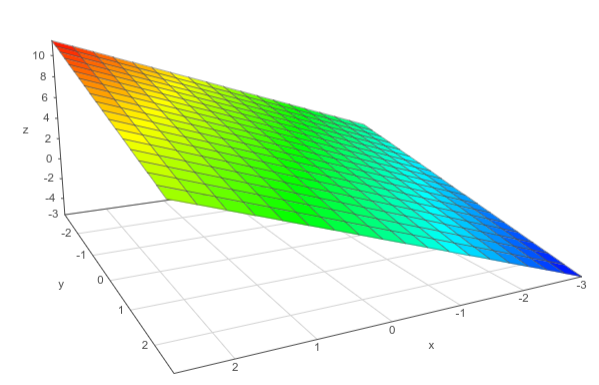
\includegraphics[scale=0.3]{figures-exercices/fpv-fiche1-exo3-fig1}	

	$f(x,y) = 2x - y + 3$		
	\end{minipage}
	\begin{minipage}{0.45\textwidth}
				\center		
				
	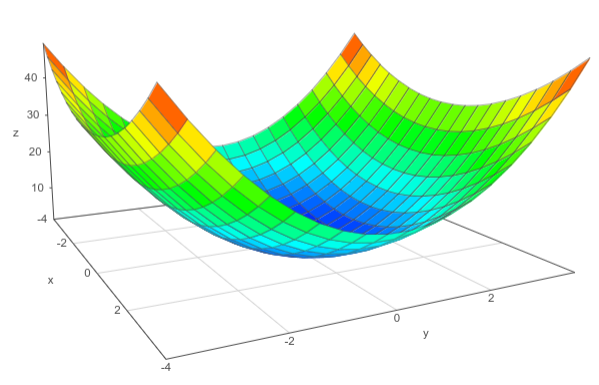
\includegraphics[scale=0.3]{figures-exercices/fpv-fiche1-exo3-fig2}	
	
	$f(x,y) = x^2 + 2y^2+1$
    \end{minipage}	
\end{center}

	\begin{center}
		\small
		\begin{minipage}{0.45\textwidth}
			\center	
			
			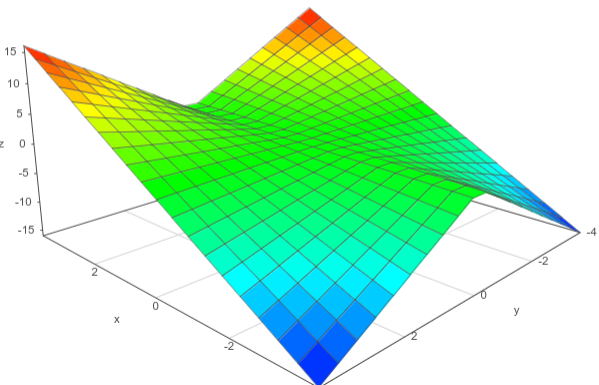
\includegraphics[scale=0.3]{figures-exercices/fpv-fiche1-exo3-fig3}	
			
			$f(x,y) = x |y|$
		\end{minipage}
		\begin{minipage}{0.45\textwidth}
			\center
				
			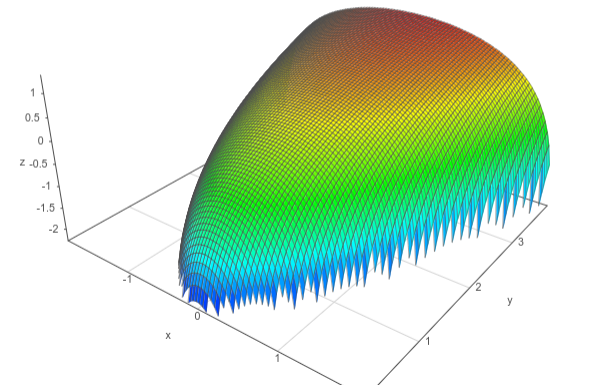
\includegraphics[scale=0.3]{figures-exercices/fpv-fiche1-exo3-fig4}
			
			$f(x,y) = \ln(y - x^2)$
		\end{minipage}	
	\end{center}
	
\begin{center}
	\small
	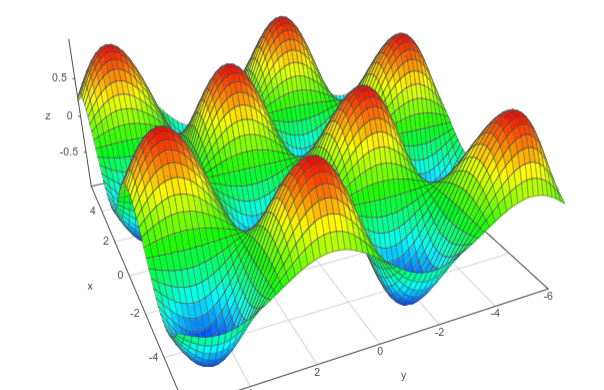
\includegraphics[scale=0.5]{figures-exercices/fpv-fiche1-exo3-fig5}
	
    $f(x,y) = \sin(x)\sin(y)$
\end{center}		
\fincorrection

\finexercice
	
		
\exercice{}
\enonce[Étude d'une fonction]
$$f(x,y) = \sqrt{x^2-2y}$$
\begin{enumerate}
	\item Déterminer, puis représenter, le domaine de définition de $f$.
	\item Tracer les lignes de niveau $(f=k)$.
    \item Tracer l'intersection du graphe de $f$ avec le plan $(x=x_0)$. Même question avec $(y=y_0)$.
    \item Représenter le graphe de $f$.
    \item Déterminer l'image de $f$.
\end{enumerate}
\finenonce

\noindication

\correction
\begin{enumerate}
	\item $\mathcal{D}_f = \{ (x,y) \in \Rr^2 \mid x^2-2y \ge 0 \}$.
	Il s'agit donc de l'ensemble des points situés sous la parabole d'équation $y = \frac{x^2}{2}$.
	\begin{center}
\begin{minipage}{0.45\textwidth}
\begin{tikzpicture}[scale=1]	
	\fill[ultra thick, color=green!70!black!40,domain=-2:2,samples=100,smooth] plot (\x,0.5*\x*\x) -- (2,-2) -- (-2,-2) -- cycle;			
	%		\fill[red!10] (0,0) circle (2);		
	
	\draw[->,>=latex, gray] (-2.2,0)--(2.5,0) node[below,black] {$x$};
	\draw[->,>=latex, gray] (0,-2.5)--(0,2.5) node[right,black] {$y$};
	
	
	
	\draw[ultra thick, color=green!70!black,domain=-2:2,samples=100,smooth] plot (\x,0.5*\x*\x) node[right,black]{$y=\frac{x^2}{2}$};	
	
	
	\fill (0,0) circle (2pt);	
	\node at (0,0)[below right] {$0$};
	\node at (1,1.5){$\mathcal{D}_f$};
	
	\node at (0,-4){Domaine de définition};
\end{tikzpicture}
\end{minipage}
\begin{minipage}{0.45\textwidth}
	\begin{tikzpicture}[scale=1]	
		%\fill[ultra thick, color=green!70!black!10,domain=-2:2,samples=100,smooth] plot (\x,0.5*\x*\x) -- (2,-2) -- (-2,-2) -- cycle;			
		%		\fill[red!10] (0,0) circle (2);		
		
		\draw[->,>=latex, gray] (-2.2,0)--(2.5,0);
		\draw[->,>=latex, gray] (0,-2.5)--(0,2.5);
		
		
		
		\draw[ultra thick, color=green!70!black,domain=-2:2,samples=100,smooth] plot (\x,0.5*\x*\x) ;	
		
		\foreach \k in {0.75,1,1.25,1.5,1.75,2,2.25,2.5}{
			\draw[thick, color=black,domain=-2:2,samples=100,smooth] plot (\x,0.5*\x*\x-0.5*\k*\k) node[right,black,scale=0.6]{$k=\k$};	
		}
		
		\fill (0,0) circle (2pt);	
		\node at (0,0)[below right] {$0$};
		\node at (1,1.5){$\mathcal{D}_f$};
		
		\node at (0,-4){Lignes de niveau};
	\end{tikzpicture}
\end{minipage}
\end{center}	
	
	
	\item Pour $k < 0$, $f(x,y)=k$ n'a pas de solutions et les lignes de niveau sont donc vides.
	Pour $k\ge 0$ fixé, $f(x,y)=k \iff x^2-2y = k^2$ est l'équation de la parabole
	$y = \frac{x^2}{2} - \frac{k^2}{2}$. C'est la même parabole que pour l'ensemble de définition mais translatée vers le bas.
	
	
	\item L'intersection du graphe de $f$ avec le plan $(x=x_0)$ est le graphe de la fonction d'une variable 	$y \mapsto f(x_0,y) = \sqrt{x_0^2-2y}$. C'est donc le graphe similaire à celui de la fonction racine carrée, mais renversé et décalé vers la droite.
	
	
	L'intersection du graphe de $f$ avec le plan $(y=y_0)$ est le graphe de $x \mapsto f(x,y_0) = \sqrt{x^2-2y_0}$. Pour $x$ grand, $f(x,y_0) \simeq \sqrt{x^2} = |x|$. On obtient deux asymptotes obliques en $\pm\infty$.

\begin{center}
	\small
\begin{tikzpicture}[scale=0.8]	
	
	\begin{scope}
		\draw[->,>=latex, gray] (-4.2,0)--(2.5,0) node[below,black] {$y$};
		\draw[->,>=latex, gray] (0,-0.5)--(0,3.5) node[right,black] {$f(x_0,y)$};
		
		
		
		\draw[ultra thick, color=blue,domain=-4:1,samples=100,smooth] plot (\x,{sqrt(2-2*\x)} );	
		
		
		\fill (1,0) circle (2pt);	
		\node at (1,0)[below] {$\frac{x_0^2}{2}$};
		
		\node at (0,-4){Tranche à $x_0$ constant};
	\end{scope}
	\begin{scope}[xshift=9cm]
		\draw[->,>=latex, gray] (-4.2,0)--(3.5,0) node[below,black] {$x$};
		\draw[->,>=latex, gray] (0,-0.5)--(0,3.5) node[right,black] {$f(x,y_0)$};
		
		
		\draw[ultra thick, color=orange,domain=-3:-1,samples=100,smooth] plot (\x,{sqrt((\x*\x)-1)} );	
		\draw[ultra thick, color=orange,domain=1:3,samples=100,smooth] plot (\x,{sqrt(\x^2-1)} );	
		
		
		\fill (1,0) circle (2pt);	
		\node[scale=0.7] at (1,0)[below] {$\sqrt{2y_0}$};
		\fill (-1,0) circle (2pt);	
		\node[scale=0.7] at (-1,0)[below] {$-\sqrt{2y_0}$};
		
		\node at (0,-4){Tranche à $y_0$ constant};
	\end{scope}
	
\end{tikzpicture}
\end{center}
	
	
	\item Voici deux points de vue du graphe de $f$.
	
\begin{center}
	\hspace*{-2cm}
		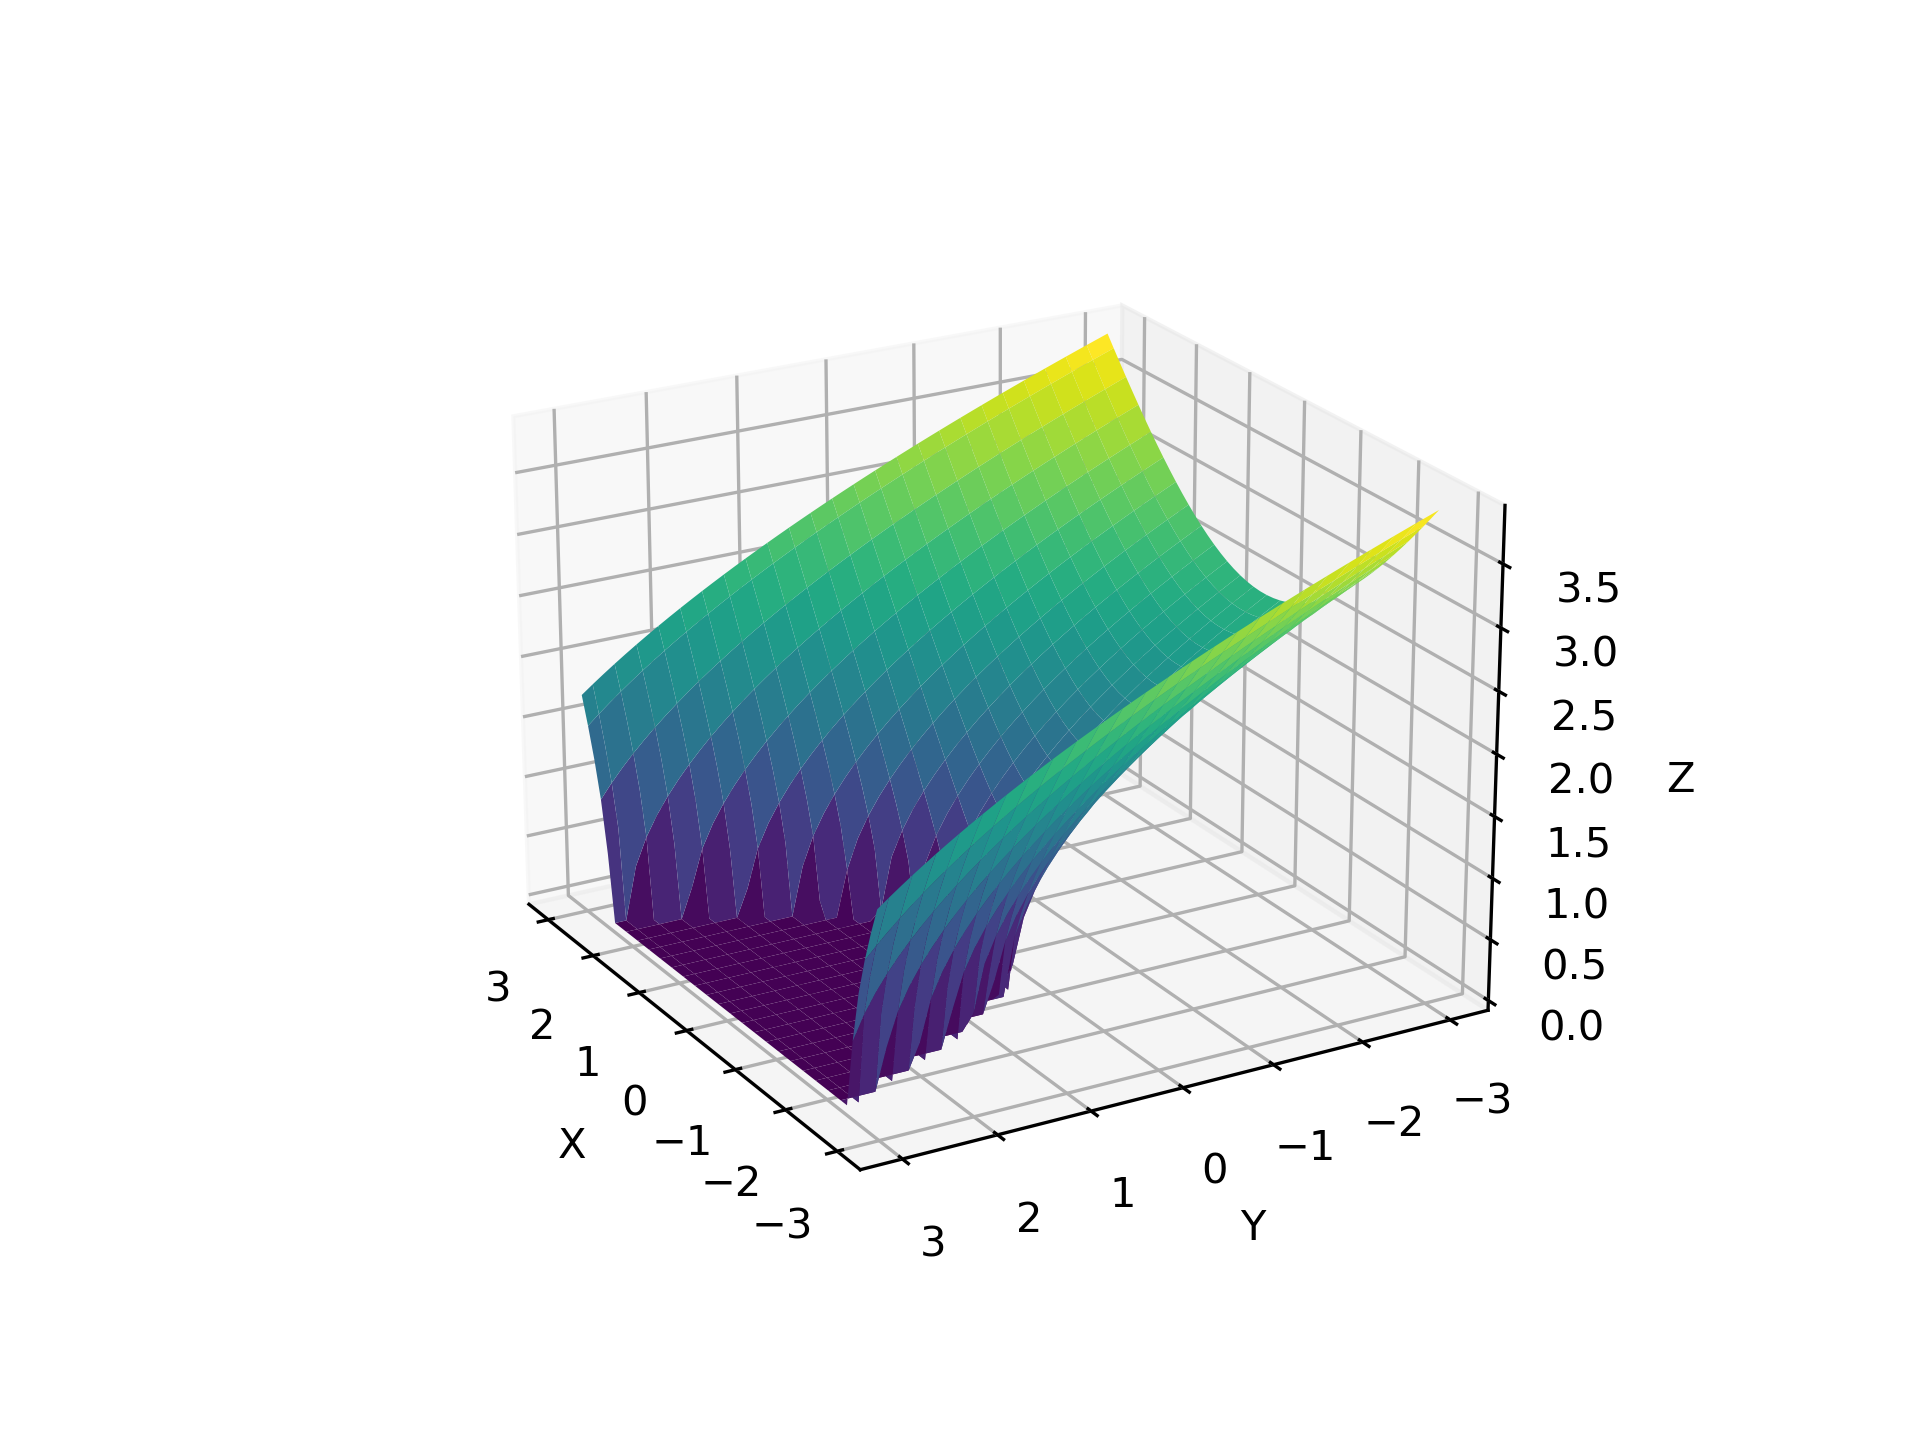
\includegraphics[scale=0.6]{figures-exercices/fpv-fiche1-exo4-fig1}			
	\hspace*{-2cm}
		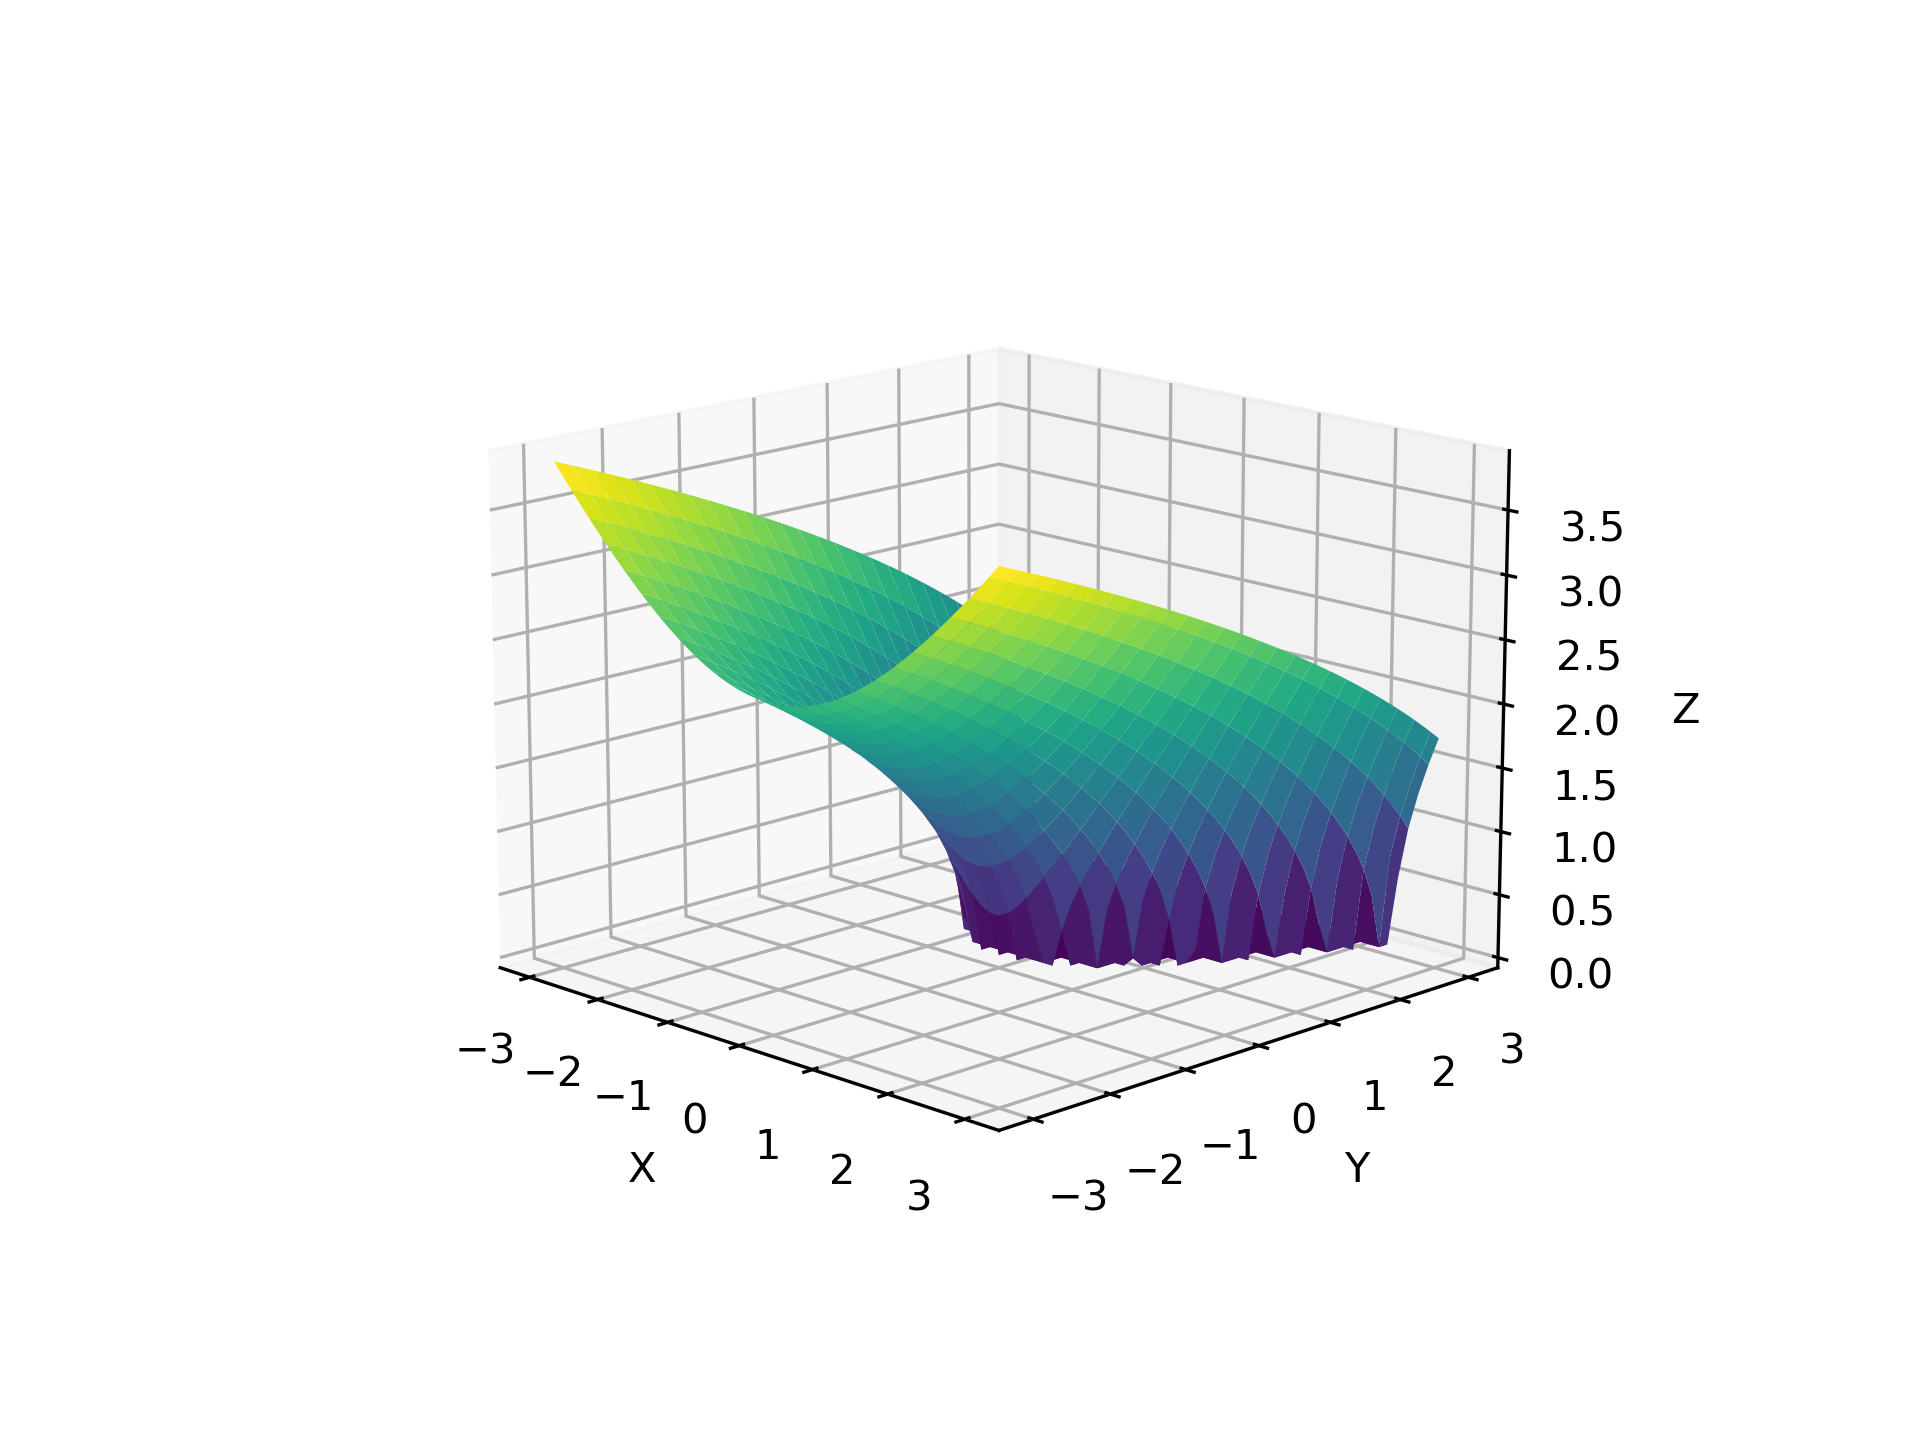
\includegraphics[scale=0.6]{figures-exercices/fpv-fiche1-exo4-fig2}		
\end{center}	
	
	\item L'image de $f$ est l'ensemble des valeurs possibles prises par $f$.
	On a déjà dit que ces valeurs devaient être positives : $\text{Im}\, f \subset [0,+\infty[$.
	Réciproquement si $z \ge 0$, alors en posant $(x,y) = (z,0)$ on a $f(x,y)=z$.
	Ainsi $\text{Im}\, f = [0,+\infty[$.
\end{enumerate}
\fincorrection
\finexercice

	
\exercice{}
\enonce[Lignes de niveau]
Déterminer et représenter la ligne de niveau $(f(x,y)=k)$ dans chacun des cas suivants.
\begin{enumerate}
	\item $f(x,y) = (x-y)^2$, $k=2$
	\item $f(x,y) = \arctan(x+3y)$, $k=\frac\pi4$
	\item $f(x,y) = 2x^2 + y^2$, $k=4$
	\item $f(x,y) = x^2-y^2$, $k = -1$
\end{enumerate}
\finenonce

\indication
\begin{enumerate}
	\item Deux droites.
	\item Une droite.
	\item Une ellipse.
	\item Une hyperbole.
\end{enumerate}
\finindication

\correction
\begin{enumerate}
	\item $f(x,y) = (x-y)^2$. 
	
	$f(x,y)=2 \iff (x-y)^2=2 \iff x-y = \pm \sqrt2$.
	
	La ligne de niveau est donc l'union des deux droites parallèles d'équation $x-y=+\sqrt2$ et $x-y=-\sqrt2$.
	
	\item $f(x,y) = \arctan(x+3y)$. 
	
	$f(x,y)=\frac\pi4 \iff \arctan(x+3y)=\frac\pi4 \iff x+3y = \tan(\frac\pi4) \iff x+3y=1$. 
	
	La ligne de niveau est la droite d'équation $x+3y=1$.
	
	\begin{center}
		\small
		\begin{minipage}{0.45\textwidth}	
			\begin{tikzpicture}[scale=1]	
					
					
					\draw[gray, dashed] (-2,-2) grid (2,2);
					\draw[->,>=latex, gray] (-2.5,0)--(2.5,0) node[below,black] {$x$};
					\draw[->,>=latex, gray] (0,-2.5)--(0,2.5) node[left,black] {$y$};
					
					\draw[red!70, ultra thick] (0.7,0.7+1.4142) -- (-2.2,-2.2+1.4142);
					\draw[red!70, ultra thick] (-0.7,-0.7-1.4142) -- (2.2,2.2-1.4142);
					
					\fill (0,0) circle (1pt);
					\fill (1,0) circle (1pt);
					\fill (0,1) circle (1pt);		
					
					\node at (0,0)[below left] {$0$};		
					\node at (1,0)[below left] {$1$};
					\node at (0,1)[below left] {$1$};
					
					\node at (0,-3) {$(x-y)^2=2$};
					
			\end{tikzpicture}
		\end{minipage}
		\begin{minipage}{0.45\textwidth}						
			\begin{tikzpicture}[scale=1]
					
					\draw[gray, dashed] (-2,-2) grid (2,2);
					\draw[->,>=latex, gray] (-2.5,0)--(2.5,0) node[below,black] {$x$};
					\draw[->,>=latex, gray] (0,-2.5)--(0,2.5) node[left,black] {$y$};
					
					\draw[red!70, ultra thick] (-2,{(1+2)/3}) -- (2,{(1-2)/3});
					
					
					\fill (0,0) circle (1pt);
					\fill (1,0) circle (1pt);
					\fill (0,1) circle (1pt);		
					
					\node at (0,0)[below left] {$0$};		
					\node at (1,0)[below left] {$1$};
					\node at (0,1)[below left] {$1$};
					
					\node at (0,-3) {$\arctan(x+3y)=\frac\pi4$};
			\end{tikzpicture}
		\end{minipage}
	\end{center}
	
			
	
	\item $f(x,y) = 2x^2 + y^2$. 
	
	$f(x,y) = 4 \iff 2x^2+y^2 = 4 \iff \frac{x^2}{\sqrt2 ^2}  + \frac{y^2}{2^2} = 1$.
	
	On sait (ou on devrait savoir) que $\frac{x^2}{a^2} + \frac{y^2}{b^2} = 1$ est l'équation de l'ellipse centrée en $(0,0)$ et de demi-grand axe $a$ (rayon horizontal) et demi-petit axe $b$ (rayon vertical).
	
	Il s'agit donc ici de l'ellipse ayant pour demi-axes $\sqrt2$ et $2$, centrée à l'origine.
	
		\begin{center}
		\small
		\begin{tikzpicture}[scale=1]
			
			\begin{scope}[scale=0.7]
				%\draw[gray, dashed] (-2,-2) grid (2,2);
				\draw[->,>=latex, gray] (-3.5,0)--(3.5,0) node[below,black] {$x$};
				\draw[->,>=latex, gray] (0,-2.5)--(0,2.5) node[left,black] {$y$};
				
				\draw[red!70, ultra thick]  (0,0) ellipse (3cm and 2cm);
				
				\draw[<->,>=latex,blue] (0,-0.2) -- ++(3,0) node[midway,below]{$a$};
				\draw[<->,>=latex,blue] (-0.2,0) -- ++(0,2) node[midway,left]{$b$};
				
				\node at (0,0)[below left] {$0$};
				
				\node at (0,-4) {Ellipse $\frac{x^2}{a^2} + \frac{y^2}{b^2} = 1$};
			\end{scope}
			
			\begin{scope}[xshift=8cm]
				\draw[gray, dashed] (-2,-2) grid (2,2);
				\draw[->,>=latex, gray] (-2.5,0)--(2.5,0) node[below,black] {$x$};
				\draw[->,>=latex, gray] (0,-2.5)--(0,2.5) node[left,black] {$y$};
				
				\draw[red!70, ultra thick]  (0,0) ellipse (1.4142cm and 2cm);
				
				\draw[<->,>=latex,blue] (0,-0.2) -- ++(1.4142,0) node[midway,below]{$\sqrt2$};
				\draw[<->,>=latex,blue] (-0.2,0) -- ++(0,2) node[midway,left]{$2$};
				
				% \fill (0,0) circle (1pt);
				% \fill (1,0) circle (1pt);
				% \fill (0,1) circle (1pt);		
				% 
				% \node at (0,0)[below left] {$0$};		
				% \node at (1,0)[below left] {$1$};
				% \node at (0,1)[below left] {$1$};
				
				\node at (0,-3) {$2x^2+y^2=4$};
			\end{scope}
		\end{tikzpicture}
	\end{center}
	
	
	\item $f(x,y) = x^2-y^2$.
	
	$f(x,y) = -1 \iff x^2-y^2=-1 \iff (x-y)(x+y)=-1$.
	
	On sait que $XY=k$ est l'équation d'une hyperbole dont les asymptotes sont les axes $X$ et $Y$.
	
	Ici il faut faire le changement de repère $X = x-y$, $Y=x+y$.
	Il s'agit donc d'une hyperbole ayant pour asymptotes les bissectrices (les droites d'équations $y=x$ et $y=-x$).
	
	
		\begin{center}
		\small
\begin{tikzpicture}[scale=1]
	
	\begin{scope}[scale=0.7]
		%\draw[gray, dashed] (-2,-2) grid (2,2);
		\draw[->,>=latex, gray] (-3.5,0)--(3.5,0) node[below,black] {$X$};
		\draw[->,>=latex, gray] (0,-3.5)--(0,3.5) node[left,black] {$Y$};
		
		\draw[ultra thick, color=red!70,domain=0.3:3,samples=100,smooth] plot (\x,1/\x);	
		\draw[ultra thick, color=red!70,domain=0.3:3,samples=100,smooth] plot (-\x,-1/\x);	
		
		\node at (0,0)[below left] {$0$};
		
		\node at (0,-4) {Hyperbole $XY=1$};
	\end{scope}
	
	\begin{scope}[xshift=8cm]
		\draw[gray, dashed] (-2,-2) grid (2,2);
		\draw[->,>=latex, gray] (-2.5,0)--(2.5,0) node[below,black] {$x$};
		\draw[->,>=latex, gray] (0,-2.5)--(0,2.5) node[left,black] {$y$};
		
		\draw[blue] (-2,-2) -- (2,2);
		\draw[blue] (-2,2) -- (2,-2);
		
		\begin{scope}[rotate=45]
			\draw[ultra thick, color=red!70,domain=0.18:3,samples=100,smooth] plot (\x,0.5/\x);	
			\draw[ultra thick, color=red!70,domain=0.18:3,samples=100,smooth] plot (-\x,-0.5/\x);	
		\end{scope}
		
		
		\fill (0,0) circle (1pt);
		\fill (1,0) circle (1pt);
		\fill (0,1) circle (1pt);		
		% 
		\node at (0,0)[below left] {$0$};		
		\node at (1,0)[below left] {$1$};
		% \node at (0,1)[below left] {$1$};
		
		\node at (0,-3) {$x^2-y^2=-1$};
	\end{scope}
\end{tikzpicture}
	\end{center}
\end{enumerate}

\fincorrection
\finexercice


\exercice{}
\enonce[Lignes de niveau]
Répondez graphiquement aux questions à l’aide des lignes de niveau de la fonction :
$$f(x,y) = -\frac{x^3}{3} - xy - y^2 + x + \frac32$$

\begin{center}
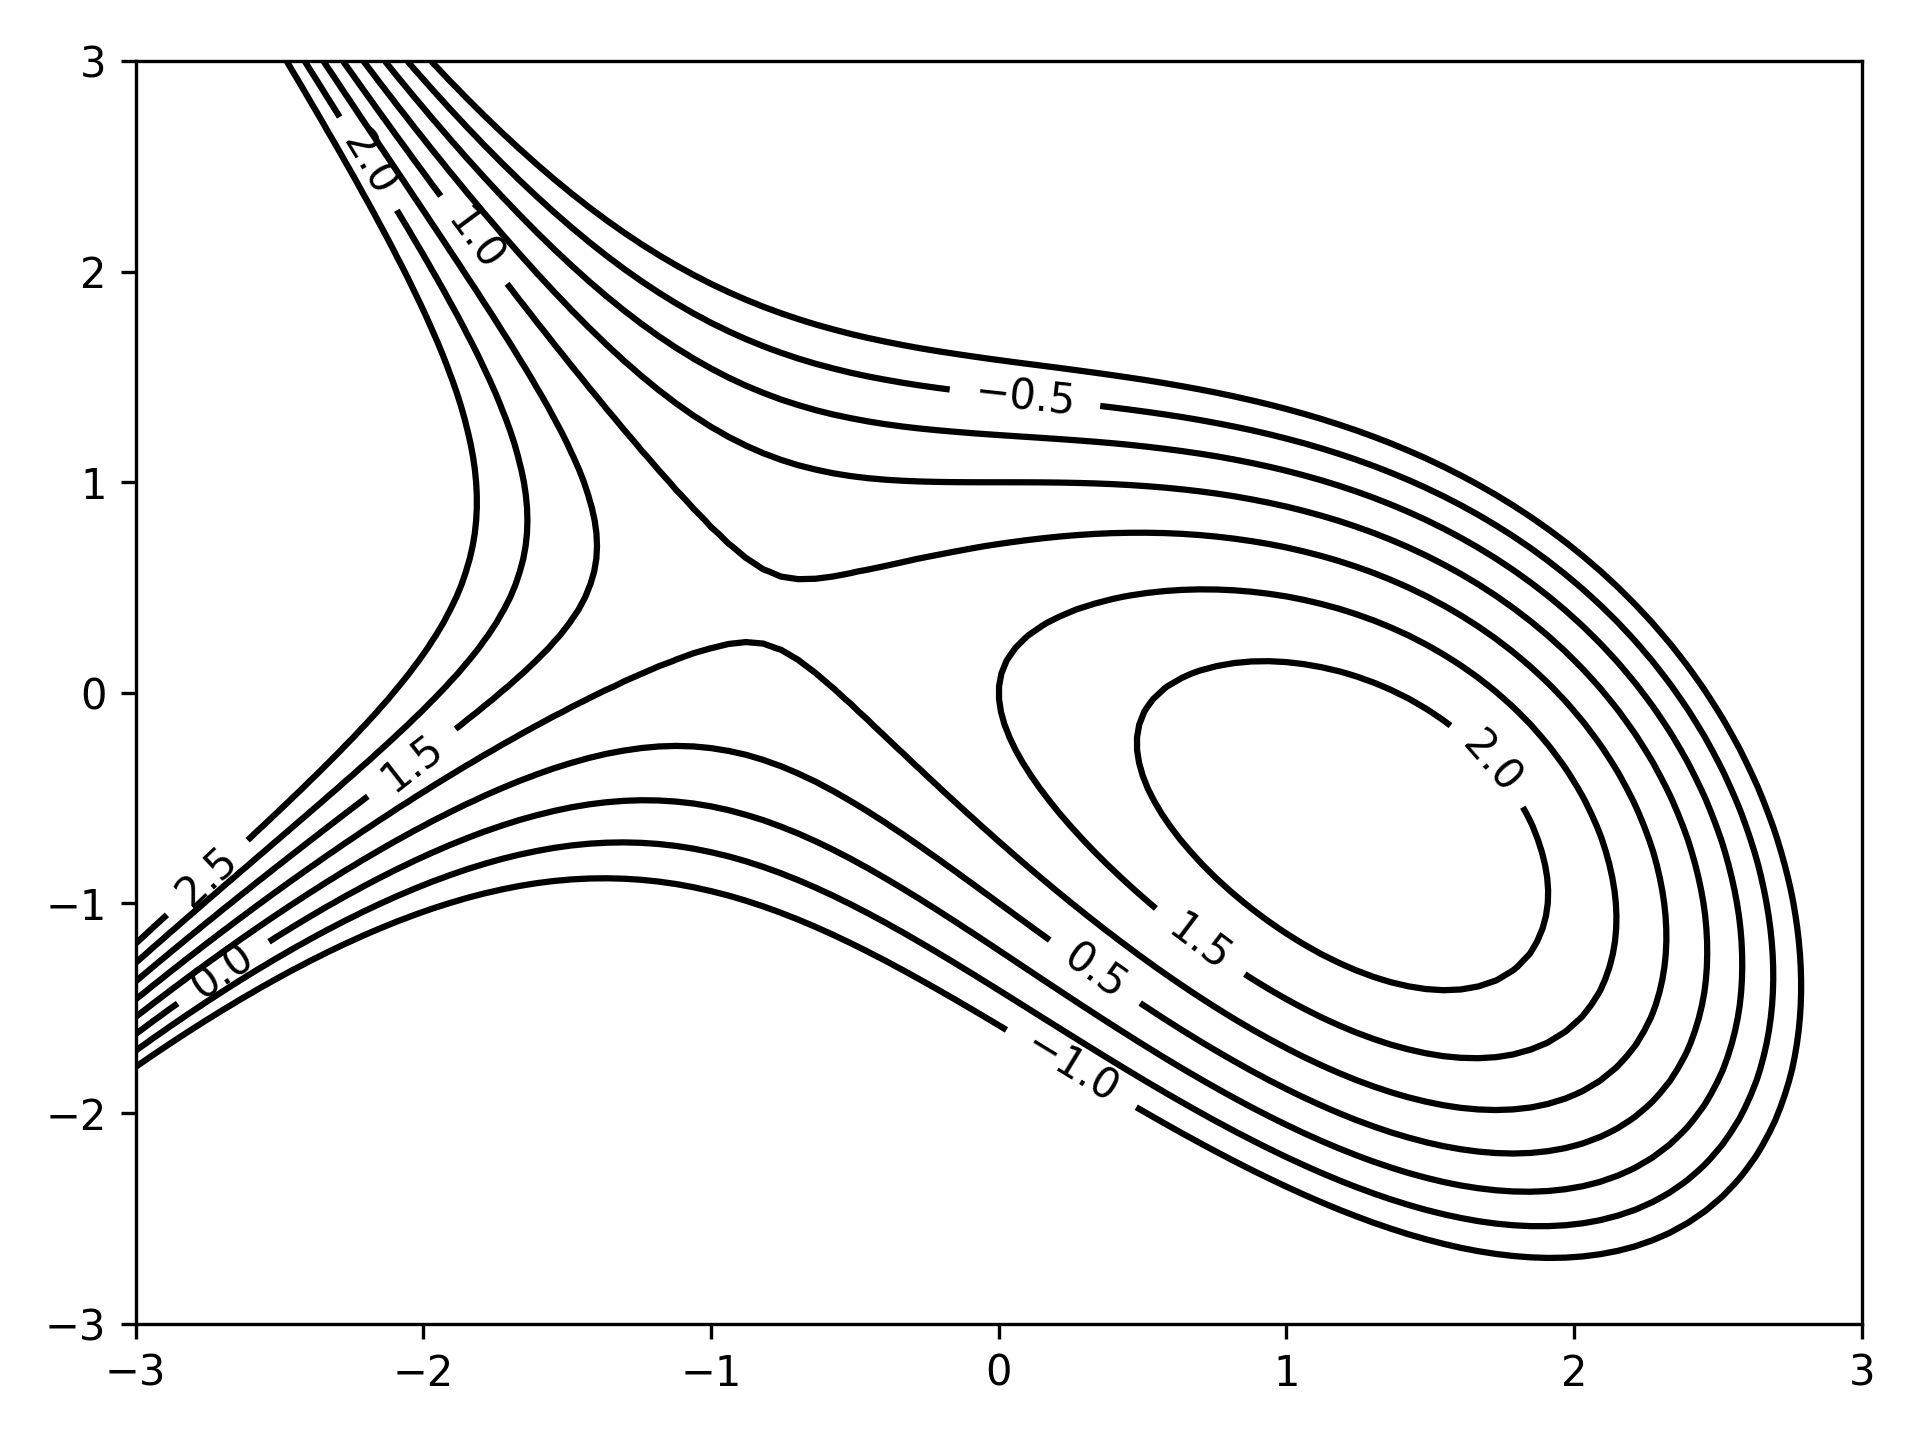
\includegraphics[scale=0.7]{figures-exercices/fonction-niveaux}
\end{center}

\begin{enumerate}
	\item Représenter le graphe de la fonction $y \mapsto f(0,y)$.	
	\item Représenter le graphe de la fonction $x \mapsto f(x,0)$.
	\item Représenter le graphe de $f$.
\end{enumerate}

\finenonce


\indication
Considérer les lignes de niveau comme une carte topographique avec des altitudes et essayer de visualiser la forme du terrain.
\finindication

\correction
On remarque que les lignes sont tracées pour des écarts de valeurs de $0.5$.
\begin{enumerate}
	\item Tracer d'abord la droite verticale d'équation $(x=0)$ sur le graphique. Il s'agit de comprendre comment varie $f(0,y)$ lorsque on se déplace sur cette droite.
	On part du bas de la droite, la première ligne rencontrée a pour niveau $-1$ (pour $y \simeq -1.5$) ; puis en remontant sur la droite le niveau monte jusqu'à atteindre environ $1.5$  (autour de $y=0)$  qui sera le maximum ; puis le niveau redescend jusqu'au niveau $-1$ (pour $y \simeq 1.7$).
	
	\item Pour $x \mapsto f(x,0)$. On trace la droite horizontale d'équation $(y=0)$. Sur cette droite, de la gauche vers la droite, on lit les niveaux de $f$. Au départ $f$ est plus grande que $2.5$, puis diminue, puis remonte, puis diminue.
	
	

\begin{center}
	\small
	\begin{tikzpicture}[scale=1]
		
		\begin{scope}
			\draw[gray, dashed] (-2,-2) grid (2,2);
			\draw[->,>=latex, gray] (-2.5,0)--(2.5,0) node[below,black] {$y$};
			\draw[->,>=latex, gray] (0,-2.5)--(0,2.5) node[right,black] {$f(0,y)$};
			
			
			\def \x{0}
			%\def\f{ -1/3*\x*\x*\x - \x*\y - \y*\y + \x + 3/2}
			\draw[ultra thick, color=green!70!black,domain=-1.9:1.9,samples=100,smooth,variable=\y] plot (\y,{-1/3*\x*\x*\x - \x*\y - \y*\y + \x + 3/2});
			
			\fill (0,0) circle (1pt);
			\fill (1,0) circle (1pt);
			\fill (0,1) circle (1pt);		
			
			\node at (0,0)[below left] {$0$};		
			\node at (1,0)[below left] {$1$};
			\node at (0,1)[below left] {$1$};
		\end{scope}
		
		
		
		\begin{scope}[xshift=8cm]
			\draw[gray, dashed] (-2,-2) grid (2,2);
			\draw[->,>=latex, gray] (-2.5,0)--(2.5,0) node[below,black] {$x$};
			\draw[->,>=latex, gray] (0,-2.5)--(0,2.5) node[right,black] {$f(x,0)$};
			
			%\let\x\relax
			\def\y{0}
			%\def\f{ -1/3*\x*\x*\x - \x*\y - \y*\y + \x + 3/2}
			\draw[ultra thick, color=red!70,domain=-2:2,samples=100,smooth,variable=\x] plot (\x,{-1/3*\x*\x*\x - \x*\y - \y*\y + \x + 3/2});
			
			\fill (0,0) circle (1pt);
			\fill (1,0) circle (1pt);
			\fill (0,1) circle (1pt);		
			
			\node at (0,0)[below left] {$0$};		
			\node at (1,0)[below left] {$1$};
			\node at (0,1)[below left] {$1$};
		\end{scope}
	\end{tikzpicture}
\end{center}

  \item Il s'agit donc d'une sorte de selle de cheval avec en plus un maximum local	au-dessus du point $(x_0,y_0) \simeq (1.5,-0.5)$.
	
\end{enumerate}

\begin{center}
	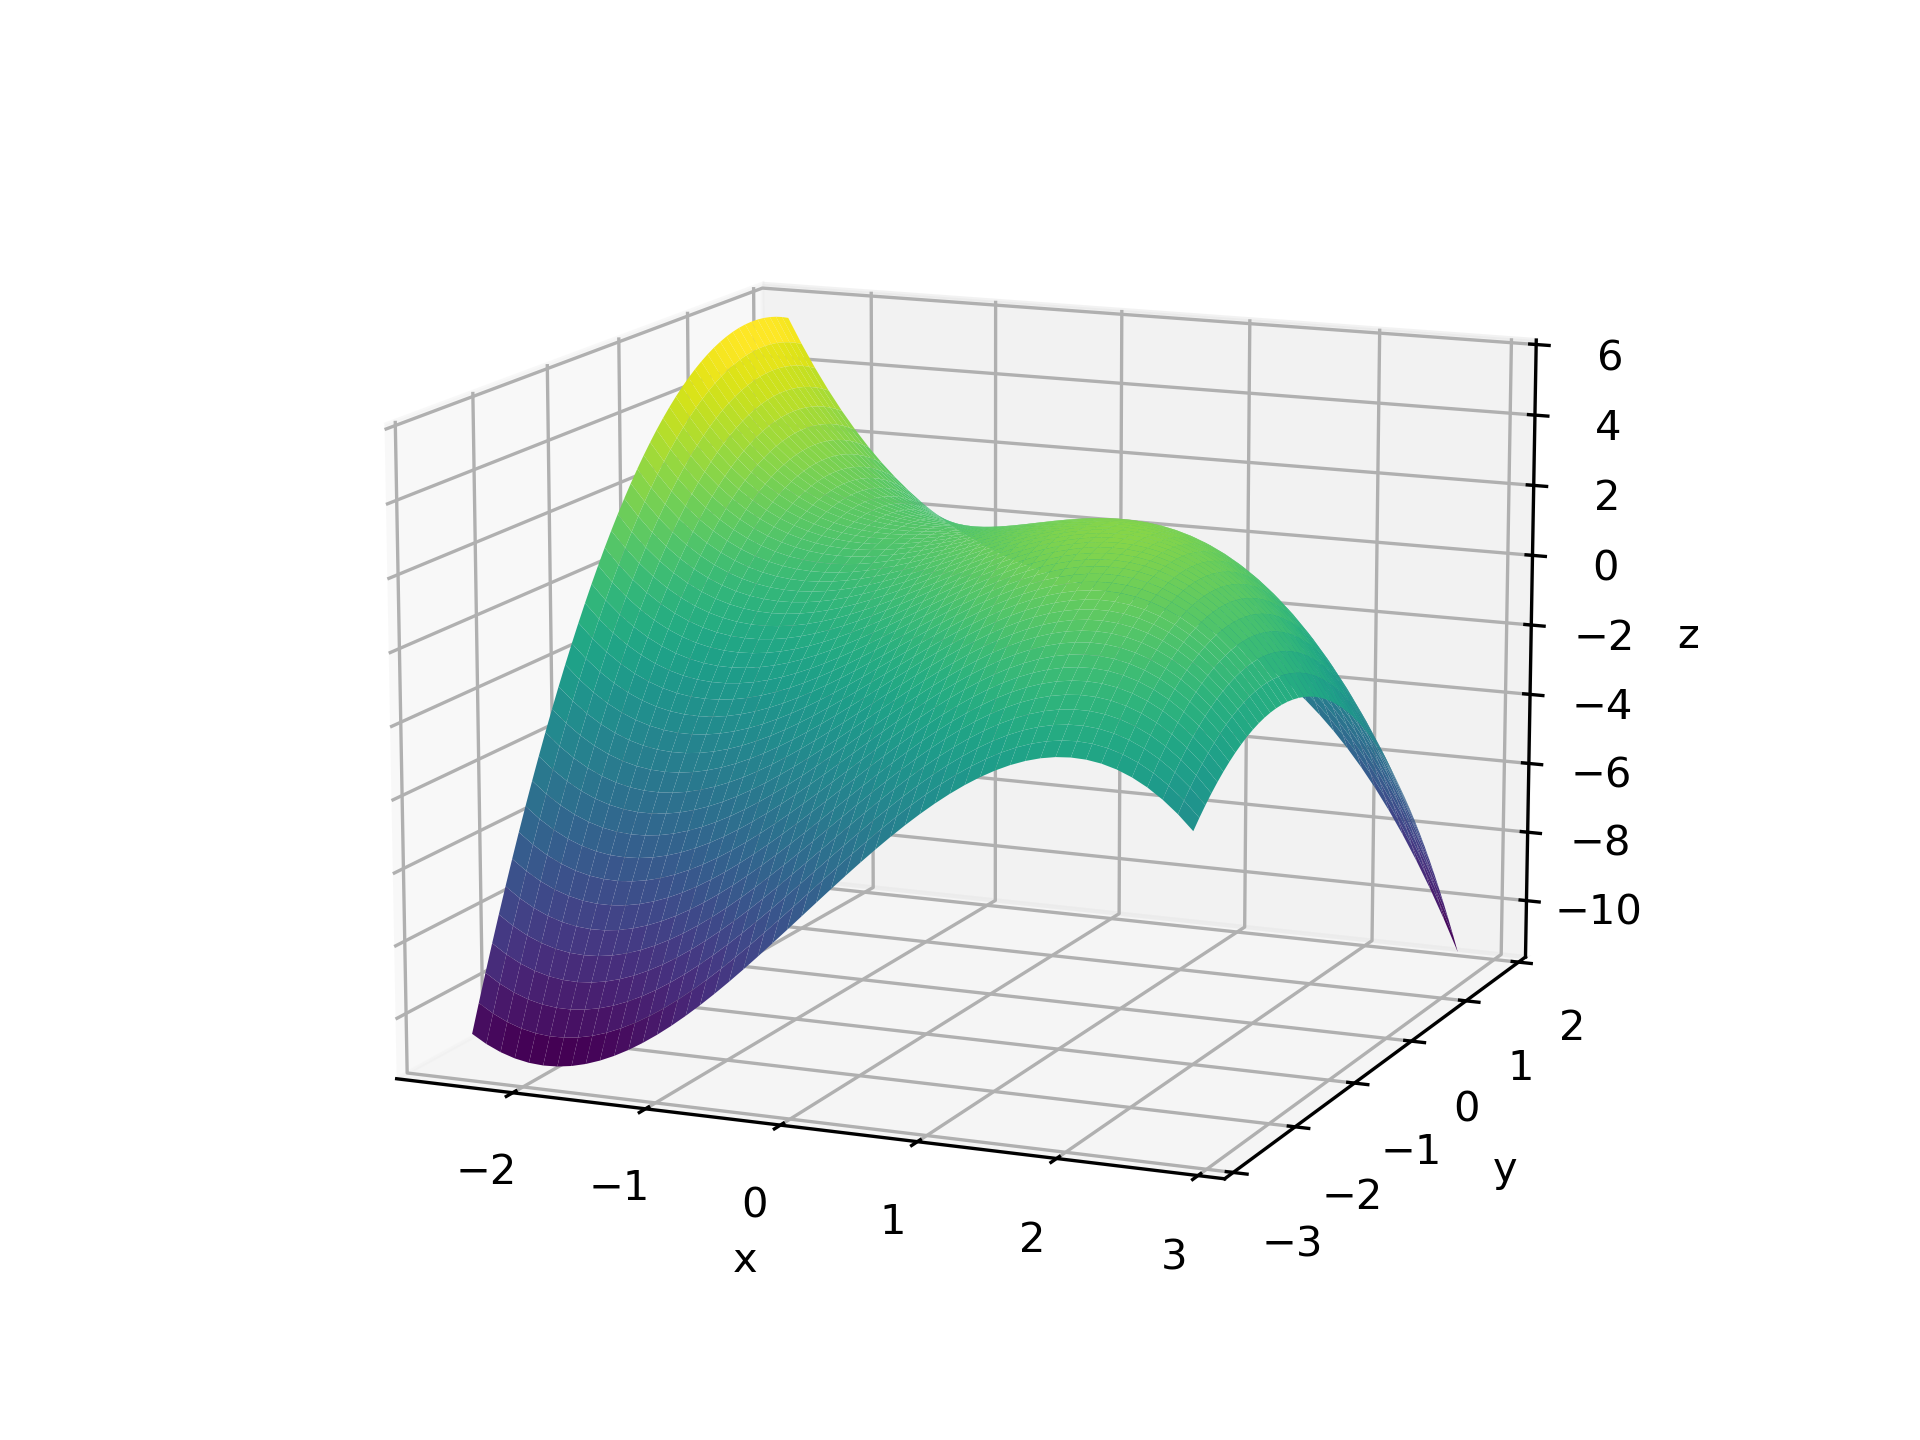
\includegraphics[scale=0.7]{figures-exercices/fonction-niveaux-3D}
\end{center}

\fincorrection

\finexercice

	
\exercice{}
\enonce[Équation d'état de van der Waals]

L'équation d'état de van der Waals relie la température $T$, la pression $P$ et le volume $V$ d'un fluide (gaz ou liquide) :
$$\left(P+{\frac {an^{2}}{V^{2}}}\right)\!\left(V-nb\right)=nRT$$
où $a, b, R$ sont des constantes et $n$ la quantité de matière.
C'est une amélioration de la loi des gaz parfaits \og{}$PV=nRT$\fg{}.

\begin{enumerate}
	\item Exprimer la température comme une fonction de la pression et du volume.
	\item Exprimer la pression comme une fonction de la température et du volume. 
	\item Exprimer l'équation polynomiale dont le volume est solution. Quel est le degré de cette équation ? 
	\emph{Physique.} Expliquer pourquoi pour une même température et une même pression on peut avoir deux volumes différents.
\end{enumerate}

\finenonce
\noindication
\correction

\fincorrection
\begin{enumerate}
	\item Il suffit de réarranger l'équation :
	\[
	T = \frac{1}{nR} \left( P + \frac{an^2}{V^2} \right)(V - nb).
	\]
	
	\item De même :
	\[
	P = \frac{nRT}{V - nb} - \frac{an^2}{V^2}
	\]
	
	\item On multiplie l'équation initiale par $V^2$ pour obtenir :
	\[
	PV^3 - (Pnb + nRT)V^2 + a n^2 V - a n^3 b = 0
	\]
	C'est une équation polynomiale de degré $3$ d'inconnue $V$. Ainsi pour une pression $P$ et une température $T$ fixées, plusieurs solutions sont possibles pour le volume $V$. D'un point de vue mathématique il peut y avoir jusqu'à trois solutions $V$ possibles. 
	
	Dans la réalité physique il est possible d'avoir deux volumes différents pour un même couple (pression, température), une solution correspondant à une phase liquide et l'autre à une phase gazeuse du même fluide.	Ce sont les conditions de l’expérience et les valeurs antérieures qui déterminent l'état exact du fluide.
	
\end{enumerate}
\finexercice


%===========================================
\section{Coordonnées polaires}


\exercice{}

\enonce[Coordonnées polaires]
Grâce aux coordonnées polaires, tracer la courbe définie implicitement par la relation
$(x^{2} + y^{2})^{\frac32} = 2xy$.
\finenonce

\indication
Montrer que $r = \sin(2\theta)$.
\finindication

\correction
On pose $x = r\cos\theta$, $y=r\sin\theta$ avec $r\ge0$ et $\theta \in [0,2\pi[$. On a $r = \sqrt{x^2+y^2}$.
L'équation $(x^{2} + y^{2})^{\frac32} = 2xy$ devient
$r^3 = 2r^2\cos\theta\sin\theta$, ce qui équivaut (si $r\neq0$) à $r = 2\cos\theta\sin\theta$, 
c'est-à-dire :
\[
r = \sin(2\theta) \quad \text{ et } r \ge 0.
\]

On a $\sin(2\theta)$ positif pour $\theta \in [0,\frac\pi2]$ et $\theta \in [\pi,\frac{3\pi}{2}]$.
Par $\pi$-périodicité, on étudie d'abord la fonction $\theta \mapsto \sin(2\theta)$ sur l'intervalle $[0,\frac\pi2]$ (figure de gauche).

Ensuite pour chaque $\theta \in [0,\frac\pi2]$, on trace le point de coordonnées polaires $[r:\theta]$, (c'est-à-dire le point de coordonnées cartésiennes $(r\cos\theta,r\sin\theta)$) : on voit que $r=\sin(2\theta)$ croît de $0$ à $1$ sur $[0,\frac\pi4]$, puis décroît de $1$ à $0$ sur $[\frac\pi4,0]$. On obtient une boucle dans le quadrant supérieur droit ($x\ge0$, $y\ge0$). Enfin, pour $\theta \in [\pi,\frac{3\pi}{2}]$, on obtient une seconde boucle, symétrique de la première par rapport à l'origine (dans le quadrant $x\le0$, $y\le0$). 
\begin{center}
	\begin{minipage}{0.4\textwidth}	
	\begin{tikzpicture}[scale=2]
		
		\draw[->,>=latex, gray] (-0.25,0)--(2,0) node[below,black] {$\theta$};
		\draw[->,>=latex, gray] (0,-0.25)--(0,1.5);
		
		\draw[ultra thick, color=green!70!black,domain=0:pi/2,samples=100,smooth] plot (\x,{sin(deg(2*\x))}) node[above right] {$\sin(2\theta)$};
		
		\draw[dashed] (0,1) -- (1.57,1);
	
		\fill (0,0) circle (1pt);
		\fill (pi/4,0) circle (1pt);
		\fill (pi/2,0) circle (1pt);		
		\node at (0,1)[above left] {$1$};
		\node at (0,0)[below right] {$0$};		
		\node at (pi/4,0)[below] {$\frac\pi4$};
		\node at (pi/2,0)[below] {$\frac\pi2$};		
	\end{tikzpicture}
\end{minipage}
	\begin{minipage}{0.4\textwidth}	
	\begin{tikzpicture}[scale=2]
		
		\draw[->,>=latex, gray] (-1.3,0)--(1.5,0) node[below,black] {$x$};
		\draw[->,>=latex, gray] (0,-1.3)--(0,1.3) node[right,black] {$y$};
		
		
		\draw[dashed] (1,-1) -- (1,1) -- (-1,1) -- (-1,-1) -- cycle;		
		
		\draw[ultra thick, color=red!70,domain=0:pi/2,samples=100,smooth] plot ({sin(deg(2*\x))*cos(deg(\x))}, {sin(deg(2*\x))*sin(deg(\x))});
		
		\draw[ultra thick, color=red!40,domain=0:pi/2,samples=100,smooth] plot ({-sin(deg(2*\x))*cos(deg(\x))}, {-sin(deg(2*\x))*sin(deg(\x))});
		
		\fill (0,0) circle (1pt);
		\node at (1,0)[below right] {$1$};
		\node at (-1,0)[below left] {$-1$};		
		\node at (0,0)[below right] {$0$};
	\end{tikzpicture}
\end{minipage}
\end{center}
\fincorrection
\finexercice



\exercice{}

\enonce[Coordonnées de l'espace]
\sauteligne
\begin{enumerate}
	\item Déterminer les coordonnées cartésiennes $(x,y,z)$ d'un point $P$ en fonction de ses coordonnées cylindriques $(r,\theta,z$).
	
	Pour $x>0$ et $y>0$, exprimer les coordonnées cylindriques en fonction des coordonnées cartésiennes.
	
\begin{center}
\begin{minipage}{0.8\textwidth}	
  \center	
  % Source https://tex.stackexchange.com/questions/159445/
% user31034
% needs  \usepackage{tikz,tikz-3dplot}
\tdplotsetmaincoords{70}{120}
\begin{tikzpicture}[tdplot_main_coords][scale=0.75]
	\draw[thick,gray,-latex] (0,0,0) -- (6,0,0) node[anchor=north east]{$x$};
	\draw[thick,gray,-latex] (0,0,0) -- (0,6,0) node[anchor=north west]{$y$};
	\draw[thick,gray,-latex] (0,0,0) -- (0,0,6) node[anchor=south]{$z$};
	\draw [thick](0,0,0) circle (3);
	\draw [thick](0,0,4) circle (3);
	\draw [thick](1.89,-2.36,0.05) -- (1.89,-2.36,4.05);
	\draw [thick](-1.89,2.36,-0.05) -- (-1.89,2.36,4-0.05);

%	\filldraw[fill=orange, nearly transparent] (-4,-4,4) -- (4,-4,4) --  (4,5,4) -- (-4,5,4) -- (-4,-4,4);
%	\filldraw[fill=blue, nearly transparent] (0,0,4) -- (5.2,6,4) --  (5.2,6,0) -- (0,0,0) -- (0,0,4);
	\draw [thick,blue](0,0,0) -- (0,0,4);
	\filldraw [color=blue](2,2.25,4) circle (0.075cm) node[above right]{$M$};
	\filldraw [color=blue](1.98,2.29,0) circle (0.05cm) ;
	\filldraw [color=blue](0,0,4) circle (0.05cm) node[right] {$z$};

	\draw [thick,,blue,->,-latex](1.7,0,0) arc (0:48:1.7) node[midway, below]{$\theta$};
	\draw[thick, blue](0,0,0) -- (2,2.35,0) node[midway, above]{$r$};
	\draw [] (2,2.25,4)--(1.95,2.25,0);
	\draw[](0,0,4) -- (2,2.35,4);	
\end{tikzpicture}
\end{minipage}  
\end{center}
	
	\item Les coordonnées sphériques $(r, \varphi, \lambda)$ sont la donnée d'une altitude $r$, d'une latitude $\varphi$ et d'une longitude $\lambda$.
	Déterminer les coordonnées cartésiennes $(x,y,z)$ d'un point $P$ en fonction de ses coordonnées sphériques $(r, \varphi, \lambda)$.
	
	Pour $x>0$ et $y>0$, exprimer les coordonnées sphériques en fonction des coordonnées cartésiennes.
	
\begin{center}
\begin{minipage}{0.8\textwidth}	
	\center
    
    ~	
	% Stereographic and cylindrical map projections
% Author: Tomasz M. Trzeciak
% Source: LaTeX-Community.org
%         <http://www.latex-community.org/viewtopic.php?f=4&t=2111>

% Need fig_gps_3d_preamb_01.tex

\newcommand\pgfmathsinandcos[3]{%
  \pgfmathsetmacro#1{sin(#3)}%
  \pgfmathsetmacro#2{cos(#3)}%
}
\newcommand\LongitudePlane[3][current plane]{%
  \pgfmathsinandcos\sinEl\cosEl{#2} % elevation
  \pgfmathsinandcos\sint\cost{#3} % azimuth
  \tikzset{#1/.style={cm={\cost,\sint*\sinEl,0,\cosEl,(0,0)}}}
}
\newcommand\LatitudePlane[3][current plane]{%
  \pgfmathsinandcos\sinEl\cosEl{#2} % elevation
  \pgfmathsinandcos\sint\cost{#3} % latitude
  \pgfmathsetmacro\yshift{\cosEl*\sint}
  \tikzset{#1/.style={cm={\cost,0,0,\cost*\sinEl,(0,\yshift)}}} %
}
\newcommand\DrawLongitudeCircle[2][1]{
  \LongitudePlane{\angEl}{#2}
  \tikzset{current plane/.prefix style={scale=#1}}
   % angle of "visibility"
  \pgfmathsetmacro\angVis{atan(sin(#2)*cos(\angEl)/sin(\angEl))} %
  \draw[current plane] (\angVis:1) arc (\angVis:\angVis+180:1);
  \draw[current plane,dashed] (\angVis-180:1) arc (\angVis-180:\angVis:1);
}
\newcommand\DrawLatitudeCircle[2][1]{
  \LatitudePlane{\angEl}{#2}
  \tikzset{current plane/.prefix style={scale=#1}}
  \pgfmathsetmacro\sinVis{sin(#2)/cos(#2)*sin(\angEl)/cos(\angEl)}
  % angle of "visibility"
  \pgfmathsetmacro\angVis{asin(min(1,max(\sinVis,-1)))}
  \draw[current plane] (\angVis:1) arc (\angVis:-\angVis-180:1);
  \draw[current plane,dashed] (180-\angVis:1) arc (180-\angVis:\angVis:1);
}

% Latitude-longitude
\begin{tikzpicture}[scale=1]
%% some definitions

\def\R{3} % sphere radius
\def\angEl{35} % elevation angle
\def\angAz{-105} % azimuth angle
\def\angPhi{0} % longitude of point P
\def\angBeta{40} % latitude of point P

%% working planes

\pgfmathsetmacro\H{\R*cos(\angEl)} % distance to north pole
\tikzset{xyplane/.style={cm={cos(\angAz),sin(\angAz)*sin(\angEl),-sin(\angAz),
                              cos(\angAz)*sin(\angEl),(0,0)}}}
\LongitudePlane[xzplane]{\angEl}{\angAz}
\LongitudePlane[pzplane]{\angEl}{\angPhi}
\LatitudePlane[equator]{\angEl}{0}

%% draw xyplane and sphere

%\draw[xyplane] (-2*\R,-2*\R) rectangle (2.2*\R,2.8*\R);
\fill[ball color=white] (0,0) circle (\R); % 3D lighting effect
\draw (0,0) circle (\R);

%% characteristic points

\coordinate (O) at (0,0);
\coordinate (N) at (0,\H);
\coordinate (S) at (0,-\H);
\path[pzplane] (\angBeta:\R) coordinate (P);
\path[pzplane] (\R,0) coordinate (PE);
\path[xzplane] (\R,0) coordinate (XE);
\path (PE) ++(0,-\H) coordinate (Paux); % to aid Phat calculation
\coordinate (Phat) at (intersection cs: first line={(N)--(P)},
                                        second line={(S)--(Paux)});

%% draw xyz coordinate system

\draw[xyplane,<->,>=latex, thick] (2.2*\R,0) node[below] {$x$} -- (0,0) -- (0,1.5*\R)
    node[right] {$y$};
\draw[->,>=latex, thick] (0,-\H) -- (0,1.4*\R) node[above] {$z$};

%% draw lines and put labels

%\draw[dashed] (P) -- (N) +(0.3ex,0.6ex) node[above left] {$N$};
\fill[black!90] (N) circle (2pt) node[above left, black] {$N$};
\fill[black!80] (S) circle (2pt) node[below right, black] {$S$};
%\draw (P) -- (Phat) node[above right] {$\mathbf{\hat{P}}$};
\draw[thick, red] (O) -- (P);
\fill[red] (P) circle (2pt) node[above right] {$P$};
\draw[dashed, thick] (XE) -- (O) -- (PE);
\draw[pzplane,>=latex,->,very thick,blue] (0:0.5*\R) to[bend right=15]
    node[pos=0.4,right] {$\varphi$} (\angBeta:0.5*\R);
\draw[equator,>=latex,->,very thick,blue] (\angAz:0.4*\R) to[bend right=30]
    node[pos=0.4,below] {$\lambda$} (\angPhi:0.4*\R);

%% draw meridians and latitude circles

 \DrawLatitudeCircle[\R,green!50!black, very thick]{0} % equator
 \DrawLongitudeCircle[\R,green!50!black, very thick]{\angAz} % xzplane
 \draw[thick, red] (O) -- (P);
 
\draw[->,>=latex,thick,black] (-5,-3) node[left] {\'Equateur} 
to [bend right=30] (-1.5,-1.6); 

\draw[->,>=latex,thick,black] (-5,-2) node[below] {M\'eridien d'origine} 
to [bend left=20] (-0.7,0);
\end{tikzpicture}

\end{minipage}	
\end{center}	

\end{enumerate}
\finenonce

\noindication
\correction
\begin{enumerate}
	\item 
On obtient les coordonnées cartésiennes à partir des coordonnées cylindriques par les formules suivantes :
$$\left\{\begin{array}{rcl}
	x &=& r\cos(\theta) \\
	y &=& r\sin(\theta) \\	
	z &=& z
\end{array}\right.$$	
	
Les formules inverses sont similaires à celles pour les coordonnées polaires, pour $x>0$, $y\ge0$  :
$$\left\{\begin{array}{rcl}
	r &=& \sqrt{x^2+y^2} \\
	\theta &=&  \Arctan(y/x) \\
	z &=& z
\end{array}\right.$$

On a $x>0$, $y\ge0$ $\iff \theta \in [0,\frac\pi2]$.

	\item 	
$$\left\{\begin{array}{rcl}
	x & = & r \cos(\varphi) \cos(\lambda) \\
	y & = & r \cos(\varphi) \sin(\lambda) \\
	z & = & r \sin(\varphi)
\end{array}\right.$$

Les formules inverses sont, pour $x>0$, $y\ge0$ :
$$\left\{\begin{array}{rcl}
	r &=& \sqrt{x^2+y^2+z^2} \\	
	\varphi &=& \Arcsin\left(\frac z r\right) \\
	\lambda &=& \Arctan(y/x) \\
\end{array}\right.$$

On a $x>0$, $y\ge0$ $\iff \lambda \in [0,\frac\pi2]$.
\end{enumerate}
\fincorrection
\finexercice



%-------------------------------------------
\section{Limites}

% Cette fiche contient les exercices : 1787 

\exercice{1787, drutu, 2003/10/01}
\enonce[Limites]
Déterminer les limites
lorsqu'elles existent:
\begin{enumerate}
	\item $\lim_{(x,y)\to (0,0)} \frac{x}{x^2+y^2}$ 
	\item $\lim_{(x,y)\to (0,0)} \frac{(x+2y)^3}{x^2+y^2}$ 
	\item $\lim_{(x,y)\to (1,0)} \frac{\ln (x+e^y)}{\sqrt{x^2+y^2}}$ 
	\item $\lim_{(x,y)\to (0,0)} \frac{x^4+y^3-xy}{x^4+y^2}$ 
	\item $\lim_{(x,y)\to (0,0)} \frac{1-\cos(xy)}{y^2}$ 	
	\item $\lim_{(x,y)\to (0,0)} \frac{x^3y}{x^4+y^4}$ 
	\item $\lim_{(x,y)\to (0,0)} \frac{(x^2+y^2)^2}{x^2-y^2}$ 
	%	\item $\lim_{(x,y)\to (0,0)} \frac{\sin x}{\cos y-\ch x}$ 
\end{enumerate}
\finenonce
\indication 
\begin{enumerate}
	\item Réfuter l'existence de la limite à l'aide
	de l'étude de limite le long de la courbe $\gamma(t) = (t,0)$.
	
	\item Utiliser les coordonnées polaires dans le plan.
	
	\item Ce n'est pas une forme indéterminée.
	
	\item Chercher deux courbes dans le domaine de définition qui tendent vers l'origine telles que les limites, calculées le long de ces courbes, existent mais ont des valeurs distinctes.
	
	\item Utiliser les équivalents : $1-\cos u \sim \frac{u^2}{2}$ pour $u$ proche de $0$.
	
	\item Pas de limite.
	
	\item Pas de limite.	
\end{enumerate}
\finindication
\correction
\begin{enumerate}  
	\item Considérons le chemin  $\gamma(t) = (t,0)$, alors 
	$f(\gamma(t)) = f(t,0) = \frac{1}{t}$ n'a pas de limite lorsque $t \to 0$ (pensez-bien au cas $t>0$ et au cas $t<0$).
	Donc $f(x,y)$ n'a pas non plus de limite lorsque $(x,y)\to (0,0)$.
	
	
	\item On pose $x=r\cos\theta$, $y=r\sin\theta$.
	Alors $f(x,y) = f(r\cos\theta,r\sin\theta) = r(\cos \theta +2 \sin \theta)^3$.
	Mais $|\cos \theta +2 \sin \theta| \le |\cos\theta| + 2 |\sin\theta| \le 3$  d'où
	$| f(x,y) | \le 3^3 r$. Lorsque $(x,y) \to 0$ alors $r\to 0$ donc 
	\[
	\lim_{(x,y)\to (0,0)} \frac{(x+2y)^3}{x^2+y^2} =0.
	\]
	
	\item  
	$\lim_{(x,y)\to (1,0)} {\sqrt{x^2+y^2}} =1 \ne 0$ et
	$\lim_{(x,y)\to (1,0)} {\ln (x+e^y)}=\ln 2$. Nous sommes en présence d'une limite qui n'est pas une forme indéterminée, d'où
	\[
	\lim_{(x,y)\to (1,0)} \frac{\ln (x+e^y)}{\sqrt{x^2+y^2}}=\ln 2. 
	\]
	
	\item 
	On pose $\gamma_1(t) = (t,0)$ et $\gamma_2(t) = (0,t)$.
	Comme $f(t,0) = 1$, alors si $f(x,y)$ admettait une limite en $(0,0)$ ce serait $1$.
	Mais d'autre part $f(0,t) = t \to 0$ (quand $t\to0$), donc si $f(x,y)$ admettait une limite en $(0,0)$ ce serait $0$. Par unicité de la limite, la limite ne peut valoir à la fois $0$ et $1$, donc $f(x,y)$ n'a pas de limite en $(0,0)$.
	
	\item Lorsque $(x,y) \to (0,0)$ on a $xy \to 0$.
	Donc $1-\cos(xy) \sim \frac12 (xy)^2$. Ainsi
	$f(x,y) \sim \frac12\frac{(xy)^2}{y^2} \sim \frac12x^2$.
	Donc $\lim_{(x,y)\to (0,0)} f(x,y) =0$.
	
	\item On pose $\gamma_1(t) = (t,0)$ et $\gamma_2(t) = (t,t)$ et on prouve comme précédemment que $f(x,y)$ n'a pas de limite en $(0,0)$.
	
	\item $f$ n'est pas définie sur les droites d'équations $(y=x)$ et $(y=-x)$.
	C'est en prenant une courbe tangente à l'une de ces droites que l'on montre que $f(x,y)$ n'a pas de limite en $(0,0)$.
	Tout d'abord pour $\gamma_1(t) = (t,0)$ on a $f(t,0) = t^2$ donc si une limite de $f(x,y)$ existait cela devrait être $0$.
	Mais pour $\gamma_2(t) = \big(x(t),y(t)\big) = (t,t+t^4)$ (disons avec $t>0$), on a  
	$(x^2+y^2)^2 \sim 4t^4$, mais $x^2-y^2 = t^2 - (t+t^4)^2 = -2t^5-t^8 \sim -2t^5$.
	Donc sur le chemin $\gamma_2$, $f(t,t+t^4) \sim -\frac{2}{t}$ qui a pour limite $-\infty$ (lorsque $t\to0^+$).
	Bilan : $f(x,y)$ n'a pas de limite en $(0,0)$.
	
	
	
\end{enumerate}
\fincorrection
\finexercice



\exercice{1785, drutu, 2003/10/01}

\enonce[Double limite]
Soit $f \colon \R^2 \setminus \{(0,0)\} \to \R$ la fonction définie par
\[
f(x,y) = \frac{x^2y^2}{x^2y^2 + (x-y)^2} .
\]
Montrer que
\begin{equation*}
	\lim_{x\to 0} \ \lim_{y\to 0}f(x,y) = 0 \qquad \text{ et } \qquad \lim_{y\to 0} \ \lim_{x\to 0}f(x,y) = 0
%	\label{non}
\end{equation*}
mais que $\lim_{(x,y)\to (0,0)} f(x,y)$ n'existe pas.
\finenonce

\indication 
Diviser le numérateur et le dénominateur
par $x^2$ (resp. $y^2$) pour déterminer $\lim_{y\to 0}f(x,y)$
(resp. $\lim_{x\to 0}f(x,y)$). Montrer que, 
calculée le long d'une autre courbe
convenable, $\lim_{t \to 0} f(x(t),y(t))$ existe et ne vaut pas zéro.
\finindication

\correction
Fixons $x\neq 0$ : 
\[ 
\lim_{y\to 0}f(x,y) =  \lim_{y\to 0}\frac{y^2}{y^2 + (1-y/x)^2} 
=\frac{\lim_{y\to 0} y^2}{\lim_{y\to 0} y^2 + (1-y/x)^2}
=\frac{0}{1} =0
\]
Ainsi $\lim_{x\to 0} \ \lim_{y\to 0}f(x,y) = 0$.
Supposons que $f(x,y)$ admette une limite $\ell$ lorsque $(x,y) \to (0,0)$, alors nécessairement on a $\ell=0$.

De même pour $y\neq 0$ fixé $\lim_{x\to 0}f(x,y) =0$. D'où $\lim_{y\to 0} \ \lim_{x\to 0}f(x,y) = 0$.


D'autre part, en posant $x(t)=t$ et $y(t)=t$, on a
$f(x(t),y(t)) =  \frac{t^4}{t^4} =1$ d'où
$\lim_{t\to 0}f(x(t),y(t)) = 1$.
Si $f(x,y)$ admettait une limite lorsque $(x,y) \to (0,0)$, alors nécessairement cette limite vaudrait $1$.
Mais si elle existe, la limite est unique et ne peut donc pas valoir $0$ et $1$.
Conclusion : la limite de $f(x,y)$ lorsque $(x,y)\to (0,0)$ n'existe pas.

\fincorrection

\finexercice


%-------------------------------------------
\section{Fonctions continues}




\exercice{1794, drutu, 2003/10/01} % +1795

\enonce[Prolongement par continuité]
Étudier la continuité sur $\Rr^2$ des fonctions suivantes :

\begin{enumerate}	
%	\item $$f(x,y) = \left\{
%	\begin{array}{cc}
%		\frac{x^2y^2}{x^2+y^2} & \mbox{ si }(x,y) \neq (0,0) \\
%		0 & \mbox{ sinon. }
%	\end{array}
%	\right .$$
	
	
	\item $$f(x,y) = \left\{
	\begin{array}{cc}
		\frac{x^2y}{x^2+y^2} & \mbox{ si }(x,y) \neq (0,0) \\
		0 & \mbox{ sinon. }
	\end{array}
	\right .$$
	
	
	\item $$f(x,y) = \left\{
	\begin{array}{cc}
		\frac{x^4y}{x^4+y^6} & \mbox{ si }(x,y) \neq (0,0) \\
		0 & \mbox{ sinon. }
	\end{array}
	\right .$$
	
	\item $$f(x,y) = \left\{
	\begin{array}{cc}
		\frac{xy^4}{x^4+y^6} & \mbox{ si }(x,y) \neq (0,0) \\
		0 & \mbox{ sinon. }
	\end{array}
	\right .$$
	
	\item $$f(x,y) = \left\{
	\begin{array}{cc}
		y^2\sin \frac{x}{y} & \mbox{ si }y \neq 0 \\
		0 & \mbox{ sinon. }
	\end{array}
	\right .$$
	
	\item $$f(x,y) = \left\{
	\begin{array}{cc}
		xe^{\arctan \frac{y}{x}} & \mbox{ si }x \neq 0 \\
		0 & \mbox{ sinon. }
	\end{array}
	\right .$$
		
	\item $$f(x,y) = \left\{
	\begin{array}{cc}
		\frac{(x+y)^4}{x^4+y^4} & \mbox{ si }(x,y) \neq (0,0) \\
		1 & \mbox{ sinon. }
	\end{array}
	\right .$$
	
	
%	\item $$f(x,y) = \left\{
%	\begin{array}{cc}
%		\frac{|x|^3|y|^5}{(x^2+y^2)^2} & \mbox{ si }(x,y) \neq (0,0) \\
%		0 & \mbox{ sinon. }
%	\end{array}
%	\right .$$
	
	\item $$f(x,y) = \left\{
	\begin{array}{cc}
		\frac{e^{xy}-1}{x^2+y^2} & \mbox{ si }(x,y) \neq (0,0) \\
		0 & \mbox{ sinon. }
	\end{array}
	\right .$$        
\end{enumerate}
\finenonce

\indication
Prenons l'exemple de la première fonction : sur $\Rr^2 \setminus \{ (0,0) \}$ la fonction est continue comme somme, produit, quotient de fonctions continues.
Elle est continue en $(0,0)$ si et seulement la limite de $f(x,y)$, lorsque $(x,y) \to (0,0)$ est $f(0,0)$. Ainsi décider si $f$ est continue à l'origine revient à un calcul de limite.
\finindication


\correction
Toutes les fonctions sont continues là où elles sont définies par leur expression générale, comme  sommes, produits, quotients et compositions de fonctions continues. Il reste à étudier la continuité là où la fonction est définie \og{}à la main\fg{}.

\begin{enumerate}	
	\item À l'aide des coordonnées polaires, on voit facilement que $f(x,y) \to 0$ en $(0,0)$.
	Or $f(0,0)=0$ donc $f(x,y) \to f(0,0)$ lorsque $(x,y) \to (0,0)$. Ce qui est exactement la définition de $f$ continue en $(0,0)$.
	
	Bilan : $f$ est continue sur $\Rr \setminus \{ (0,0) \}$ et en $(0,0)$, donc $f$ est continue sur $\Rr^2$.
	
	\item On remarque que $x^4+y^6 \ge x^4$ donc $|f(x,y)| \le \left| \frac{x^4y}{x^4} \right| = |y|$. Comme $|y| \to 0$, alors $f(x,y) \to f(0,0)=0$ lorsque $(x,y) \to (0,0)$ et $f$ est continue à l'origine.
		
	\item Soit $\gamma(t) = (t^2,t)$ (avec $t>0$) alors $f(t^2,t) = \frac{t^5}{t^8+t^6} \sim \frac{t^5}{t^6} \sim \frac{1}{t}$ qui tend vers $+\infty$ lorsque $t\to 0^+$. Ainsi $f(x,y)$ ne peut pas tendre $f(0,0)=0$. Donc $f$ n'est pas continue à l'origine.
	
	\item Pour $y\neq 0$, $| f(x,y) | \le y^2$. Donc lorsque $(x,y) \to (x_0,0)$, on a $f(x,y) \to 0$. Donc $f$ est continue en tout point de la forme $(x_0,0)$. Ainsi $f$ est continue sur $\Rr^2$.
	
	\item On sait que $| \arctan(u) | < \frac\pi2$, donc $e^{\arctan(u)} < e^{\pi/2}$ est bornée.
	Ainsi $|f(x,y)| < |x| e^{\pi/2} \to 0$ lorsque $(x,y) \to (0,y_0)$. Ainsi $f$ est continue sur $\Rr^2$.
	
	\item Pour $\gamma(t) = (t,t)$ on trouve $f(t,t) = \frac{ (2t)^4}{2t^4} = 8$ qui ne tend pas vers $f(0,0)=1$ lorsque $t \to0$. Donc $f$ n'est pas continue en $(0,0)$.
	
	\item On sait $e^u-1 \sim u$, donc $f(x,y) \sim \frac{xy}{x^2+y^2}$ qui n'a pas de limite en $(0,0)$. Donc $f$ n'est pas continue en $(0,0)$.	
	
		
\end{enumerate}
\fincorrection

\finexercice


\exercice{1793, gourio, 2001/09/01}

\enonce[Une relation à itérer]
Trouver les fonctions $f$ continues sur $\Rr^2$ telles que :
$$\forall (x,y)\in \Rr^2 \qquad f(x,y)=f(x+y,x-y). $$
\finenonce

\indication
Montrer que $f(x,y) = f(2x,2y)$ et itérer encore. 
Utiliser la continuité en $(0,0)$ afin de montrer que $f$ est une fonction constante.
\finindication

\correction
Remarquons d'abord qu'en appliquant deux fois la relation on obtient :
\[
f(x,y)=f(x+y,x-y) = f(2x,2y).
\]
Ainsi par récurrence on prouve que $f(x,y)=f(2^nx,2^ny)$ quel que soit $n\in\Nn^*$.
En changeant $x$ en $x/2^n$ et $y$ en $y/2^n$, cette égalité devient :
\[
f(x,y)=f\left( \frac{x}{2^n}, \frac{y}{2^n} \right).
\]

Notons $c = f(0,0)$. Nous allons prouver que la fonction $f$ est nécessairement la fonction constante égale à $c$.
Fixons $(x,y) \in \Rr^2$ et notons $u_n = \left( \frac{x}{2^n}, \frac{y}{2^n} \right)$ une suite de points de $\Rr^2$ définie pour $n \ge 1$. Il est clair que $u_n$ tend vers $(0,0)$ lorsque $n$ tend vers $+\infty$ (souvenez-vous que $x$ et $y$ sont fixés).
Comme $f$ est continue en $(0,0)$ et que $u_n \to (0,0)$ alors $f(u_n) \to f(0,0)=c$ (lorsque $n \to +\infty$).

Mais on a vu que $f(u_n) = f(x,y)$ quel que soit $n\ge1$, donc la suite $( f(u_n) )_{n\ge1}$ est la suite constante égale à $f(x,y)$ et tend vers $c$. Ainsi $f(x,y)=c$.
Ce raisonnement est vrai quel que soit $(x,y)\in\Rr^2$ et donc $f$ est une fonction constante.
Réciproquement une fonction constante vérifie bien la relation de l'énoncé.
\fincorrection
\finexercice


\exercice{5900, rouget, 2010/10/16}
\enonce[$\Rr^2$ est homéomorphe à un disque ouvert]

Soit $\| \cdot \|$ une norme de $\Rr^2$ et $D=\{x\in \Rr^2  /\; \|x\| < 1\}$ le disque unité ouvert.
Montrer que 
$$\begin{array}[t]{cccc}
	f~:&\Rr^2&\longrightarrow&D\\[1ex]
	&x&\longmapsto& \dfrac{x}{1+\|x\|}
\end{array}$$ 
est un homéomorphisme. 

Vous devrez donc montrer que : (a) $f$ est bien définie, (b) est continue, (c) est bijective, (d) de bijection réciproque également continue.
\finenonce

\noindication

\correction
~
\begin{itemize}
  \item Pour tout $x\in E$, $\|f(x)\|= \frac{\|x\|}{1+\|x\|}< \frac{\|x\|+1}{\|x\|+1}=1$. Donc $f$ est bien une application de $E$ dans $D$.

  \item Si $y=0$, pour $x\in E$, $f(x)=y\Leftrightarrow \frac{1}{1+\|x\|}x=0\Leftrightarrow x=0$. Remarque : on note $0 = 0_{\Rr^2} = (0,0)$.

Soit alors $y\in D\setminus\{0\}$. Pour $x\in E$,

\begin{center}
	$f(x)=y\Rightarrow x=(1+\|x\|)y\Rightarrow\exists\lambda\in\Rr/\;x=\lambda y$.
\end{center}

Donc un éventuel antécédent de $y$ est nécessairement de la forme $\lambda y$, $\lambda\in\Rr$. Réciproquement, pour $\lambda\in\Rr$, $f(\lambda y)= \frac{\lambda}{1+|\lambda| \, \|y\|}y$ et donc

\begin{align*}\ensuremath
	f(\lambda y)=y&\Leftrightarrow \frac{\lambda}{1+|\lambda| \, \|y\|}=1\Leftrightarrow\lambda=1+|\lambda| \, \|y\|\\
	&\Leftrightarrow(\lambda\ge0\;\text{et}\;(1-\|y\|)\lambda=1)\;\text{ou}\;(\lambda<0\;\text{et}\;(1+\|y\|)\lambda=1)\\
	&\Leftrightarrow\lambda= \frac{1}{1-\|y\|}\;\text{(car $\|y\|<1$ et le second cas est exclu pour des raisons de signe)}.
\end{align*}

Dans tous les cas, $y$ admet un antécédent par $f$ et un seul à savoir $x= \frac{1}{1-\|y\|}y$. Ainsi,

\begin{center}
	$f$ est bijective et $\forall x\in D$, $f^{-1}(x)= \frac{1}{1-\|x\|}x$.
\end{center}

  \item On sait que l'application $x\mapsto\|x\|$ est continue sur $\Rr^2$. Donc l'application $x\mapsto \frac{1}{1+\|x\|}$ est continue sur $\Rr^2$ en tant qu'inverse d'une fonction continue sur $\Rr^2$ à valeurs dans $\Rr$, ne s'annulant pas sur $\Rr^2$. L'application $x\mapsto \frac{1}{1-\|x\|}$ est continue sur $D$ pour les mêmes raisons. Donc les applications $f$ et $f^{-1}$ sont continues sur $\Rr^2$ et $D$ respectivement. Ainsi on a montré que
l'application $f$ est bien un homéomorphisme.
\end{itemize}
\fincorrection
\finexercice


\bigskip

Corrections : Arnaud Bodin. Relecture : Axel Renard.

\end{document}
